 \section{ Butembo }\begin{figure}[H]\begin{subfigure}{\textwidth}  \centering  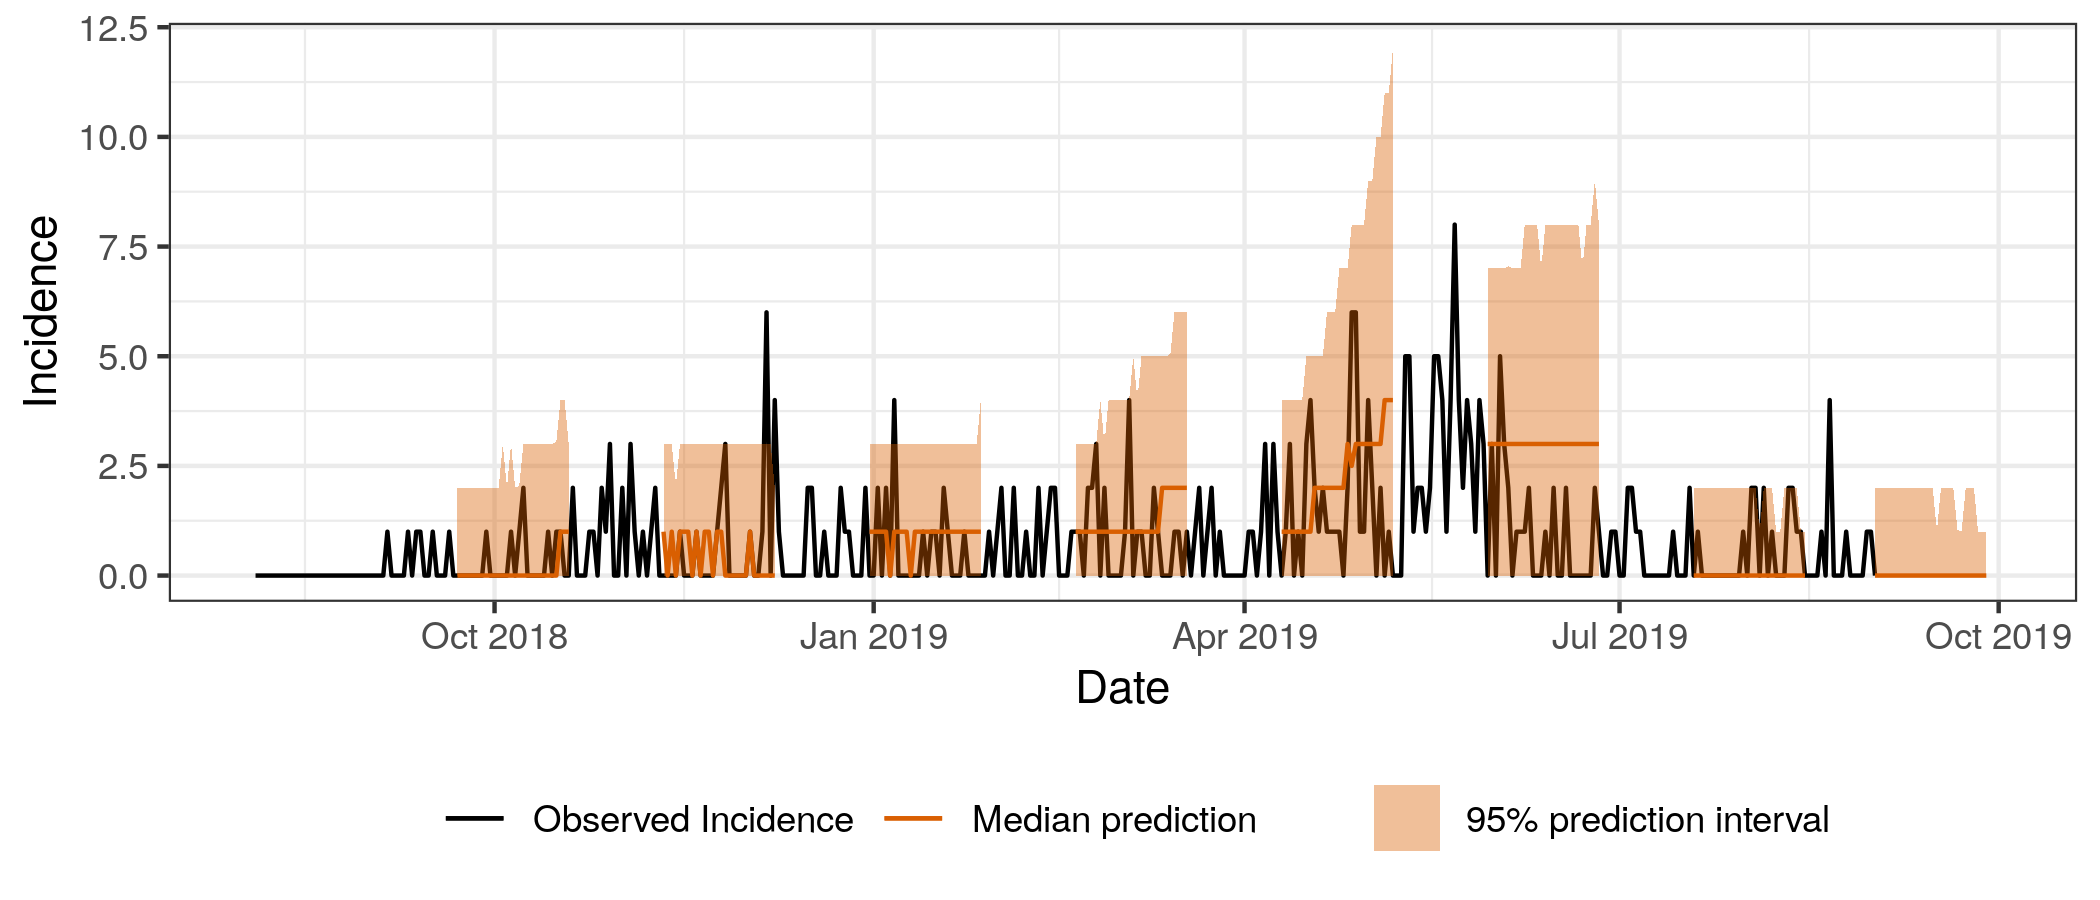
\includegraphics[width=0.9\linewidth, height=7cm]{../output/Butembo_predictions.png}  \caption{Forecasted and predicted incidence for the best fitting model}\end{subfigure}

\begin{subfigure}{\textwidth}  \centering  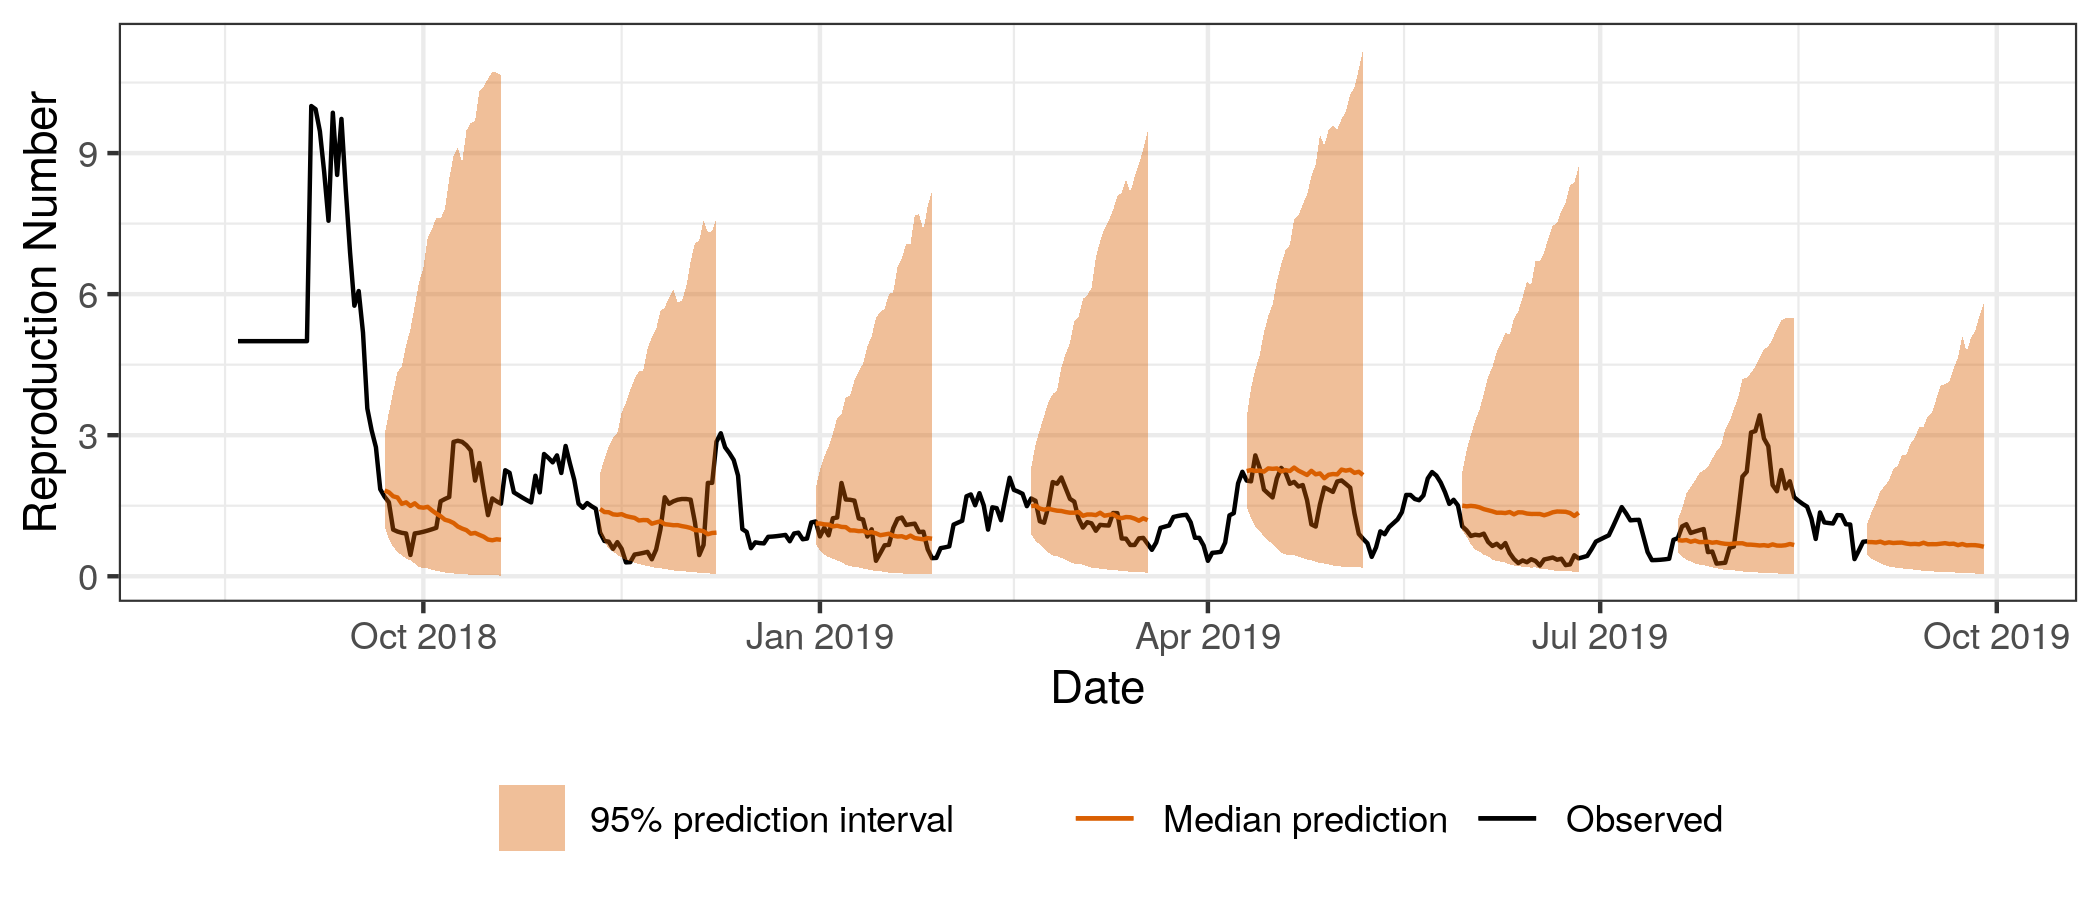
\includegraphics[width=0.9\linewidth, height=7cm]{../output/Butembo_Rs.png}  \caption{Forecasted and predicted repreoduction numbers for the best fitting model}\end{subfigure}  \caption{Median forecast with 95 \% prediction intervals and observed values for incidence and reproduction number for the best fitting model for Butembo.}\end{figure}

\begin{figure}[H]
\begin{subfigure}{0.5\textwidth}
  \centering
  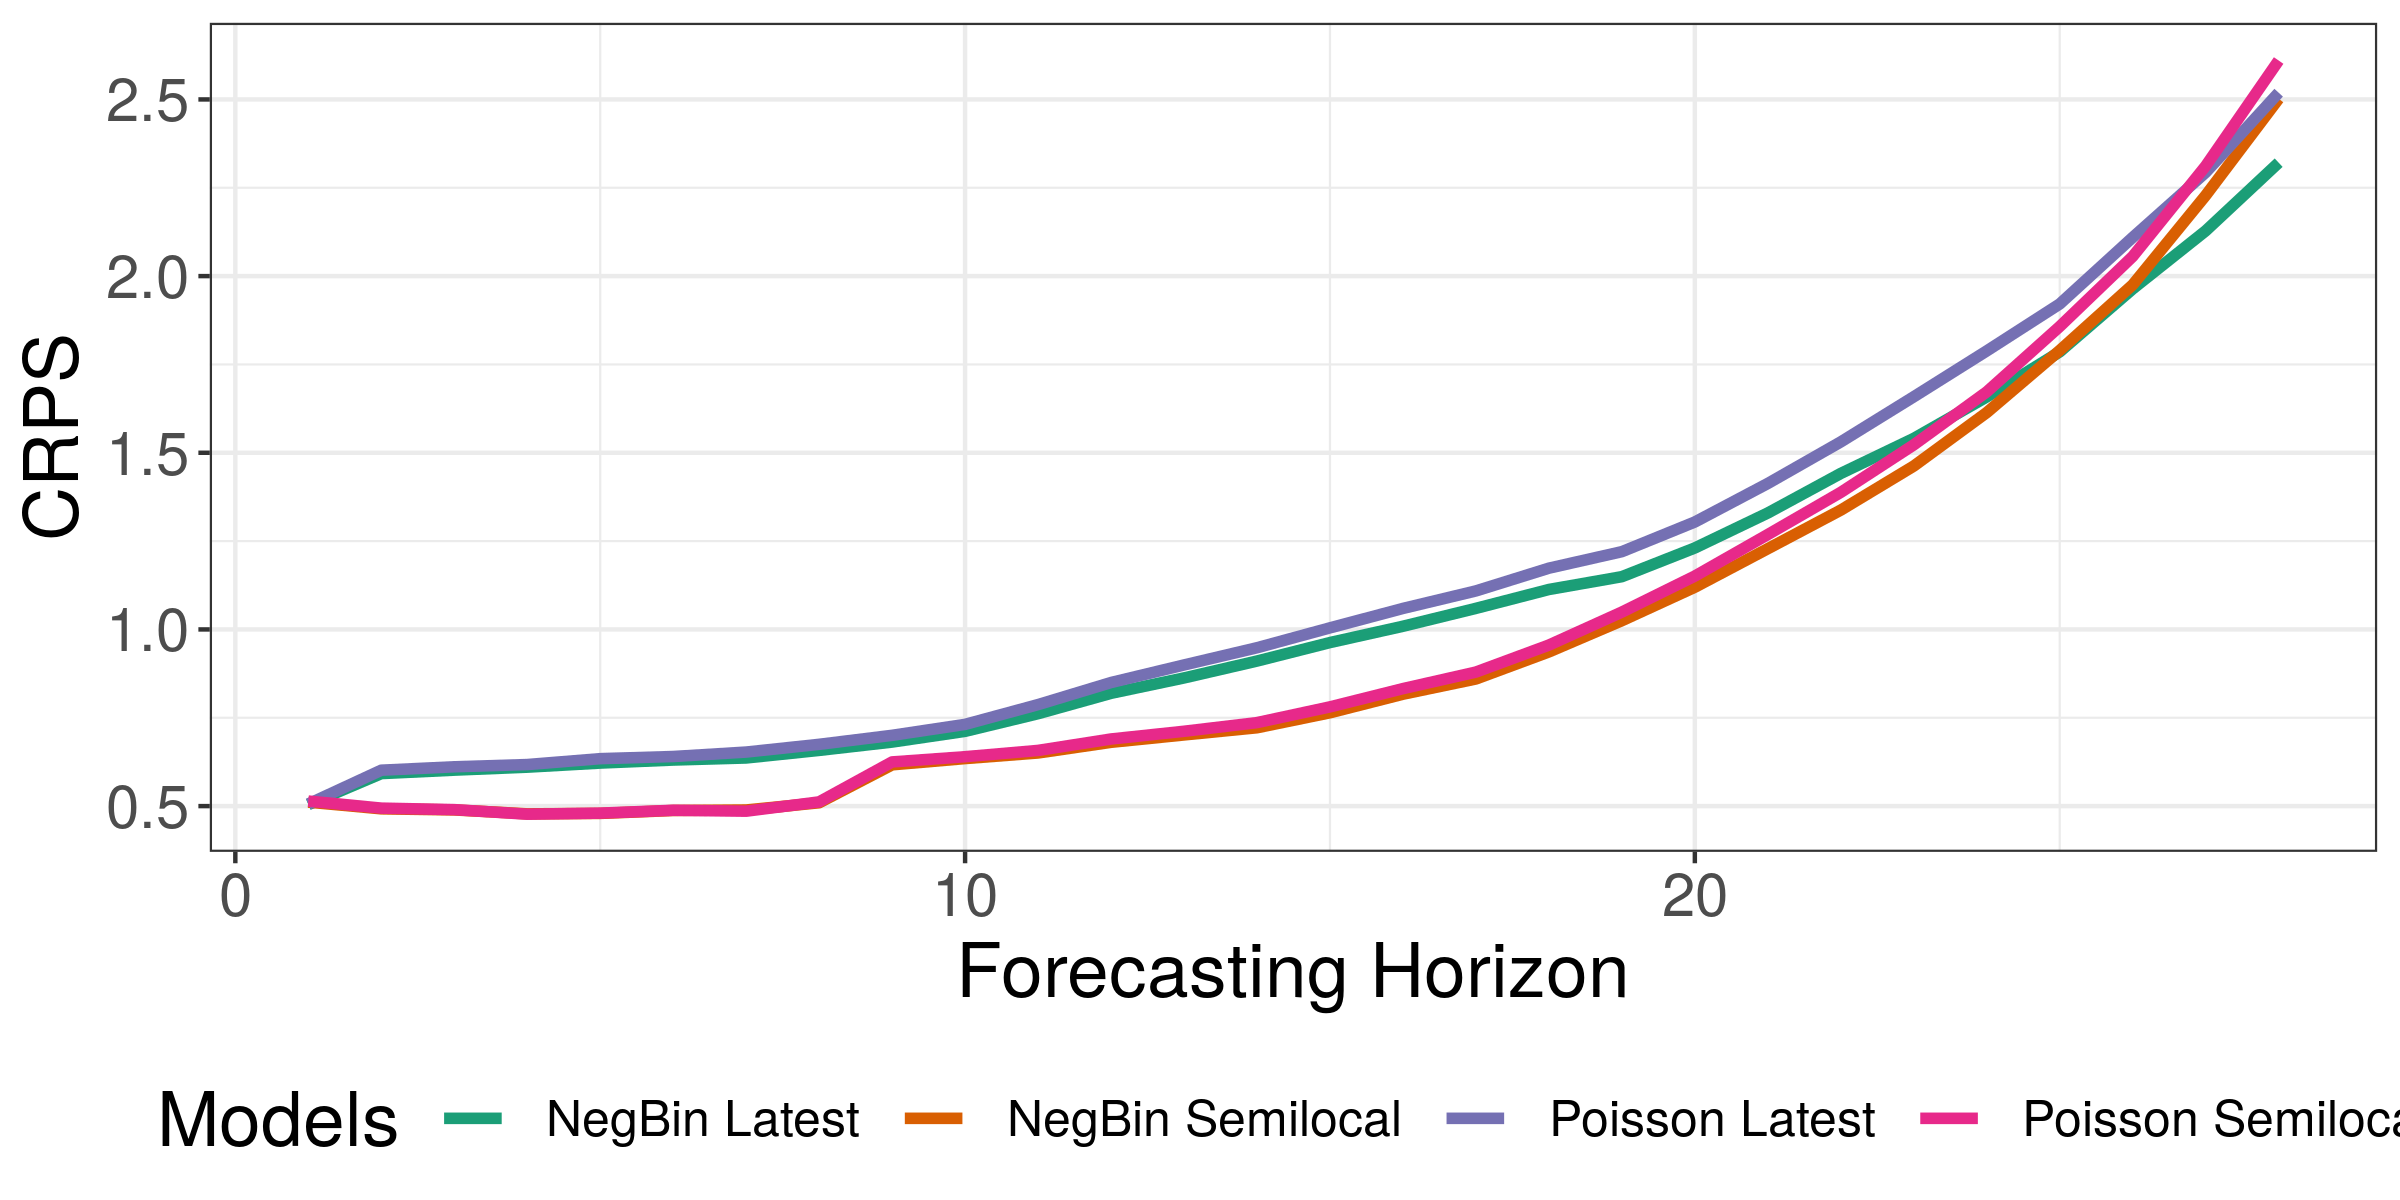
\includegraphics[width=\linewidth]{../output/Butembo_crps.png}  
  \caption{Contineously Ranked Probability Score}
  \label{Butembo_scores_1}
\end{subfigure}
\begin{subfigure}{0.5\textwidth}
  \centering
  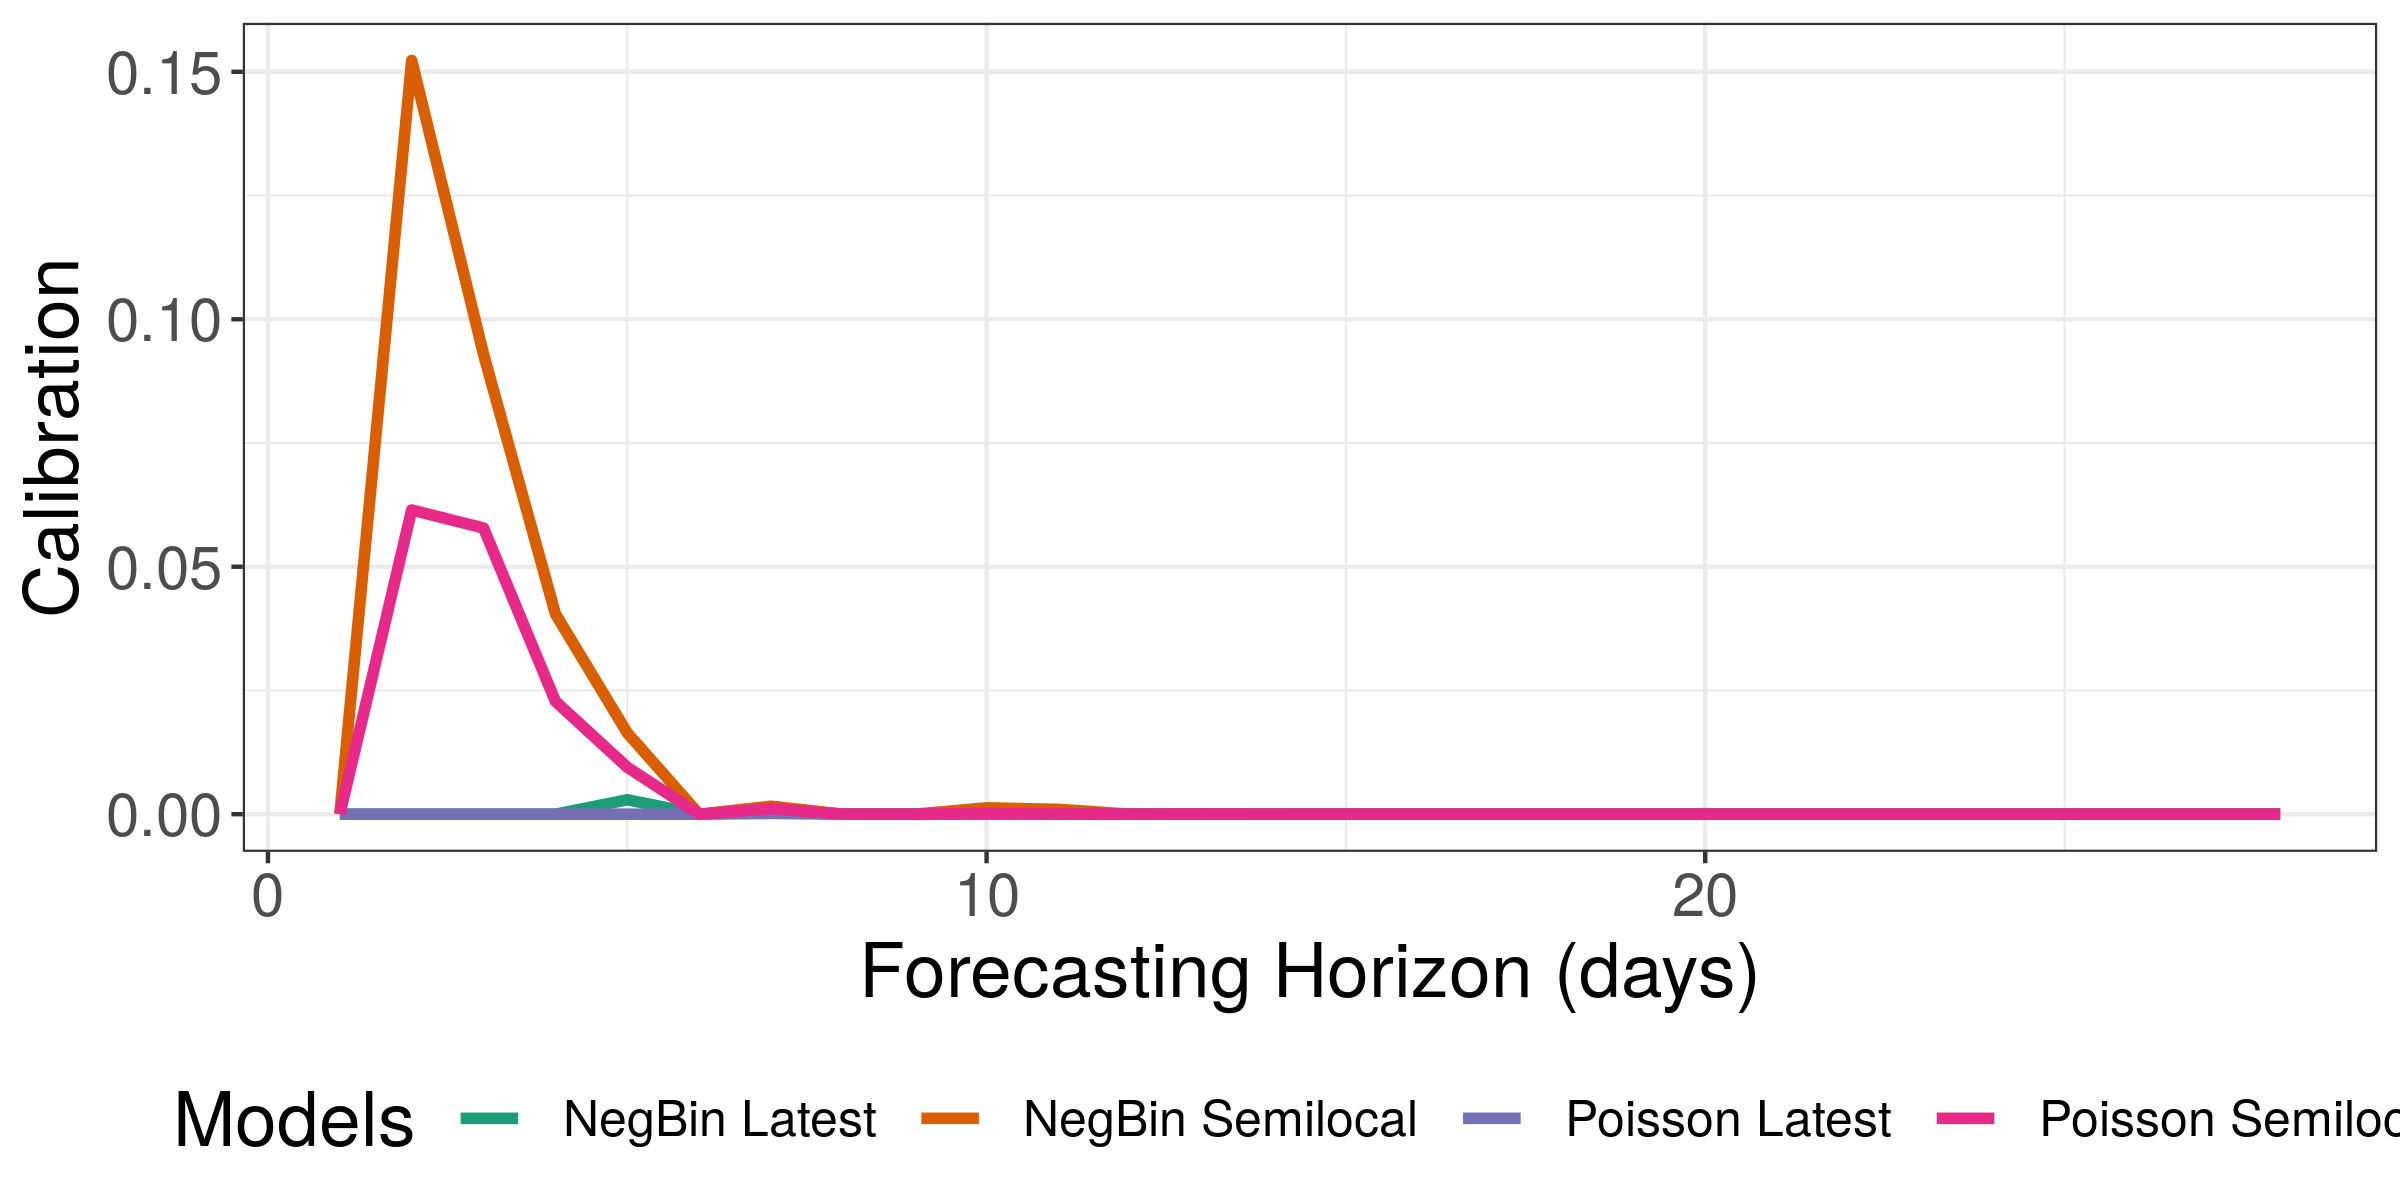
\includegraphics[width=\linewidth]{../output/Butembo_calibration.png}  
  \caption{Calibration p-value}
  \label{Butembo_scores_2}
\end{subfigure}

\begin{subfigure}{0.5\textwidth}
  \centering
  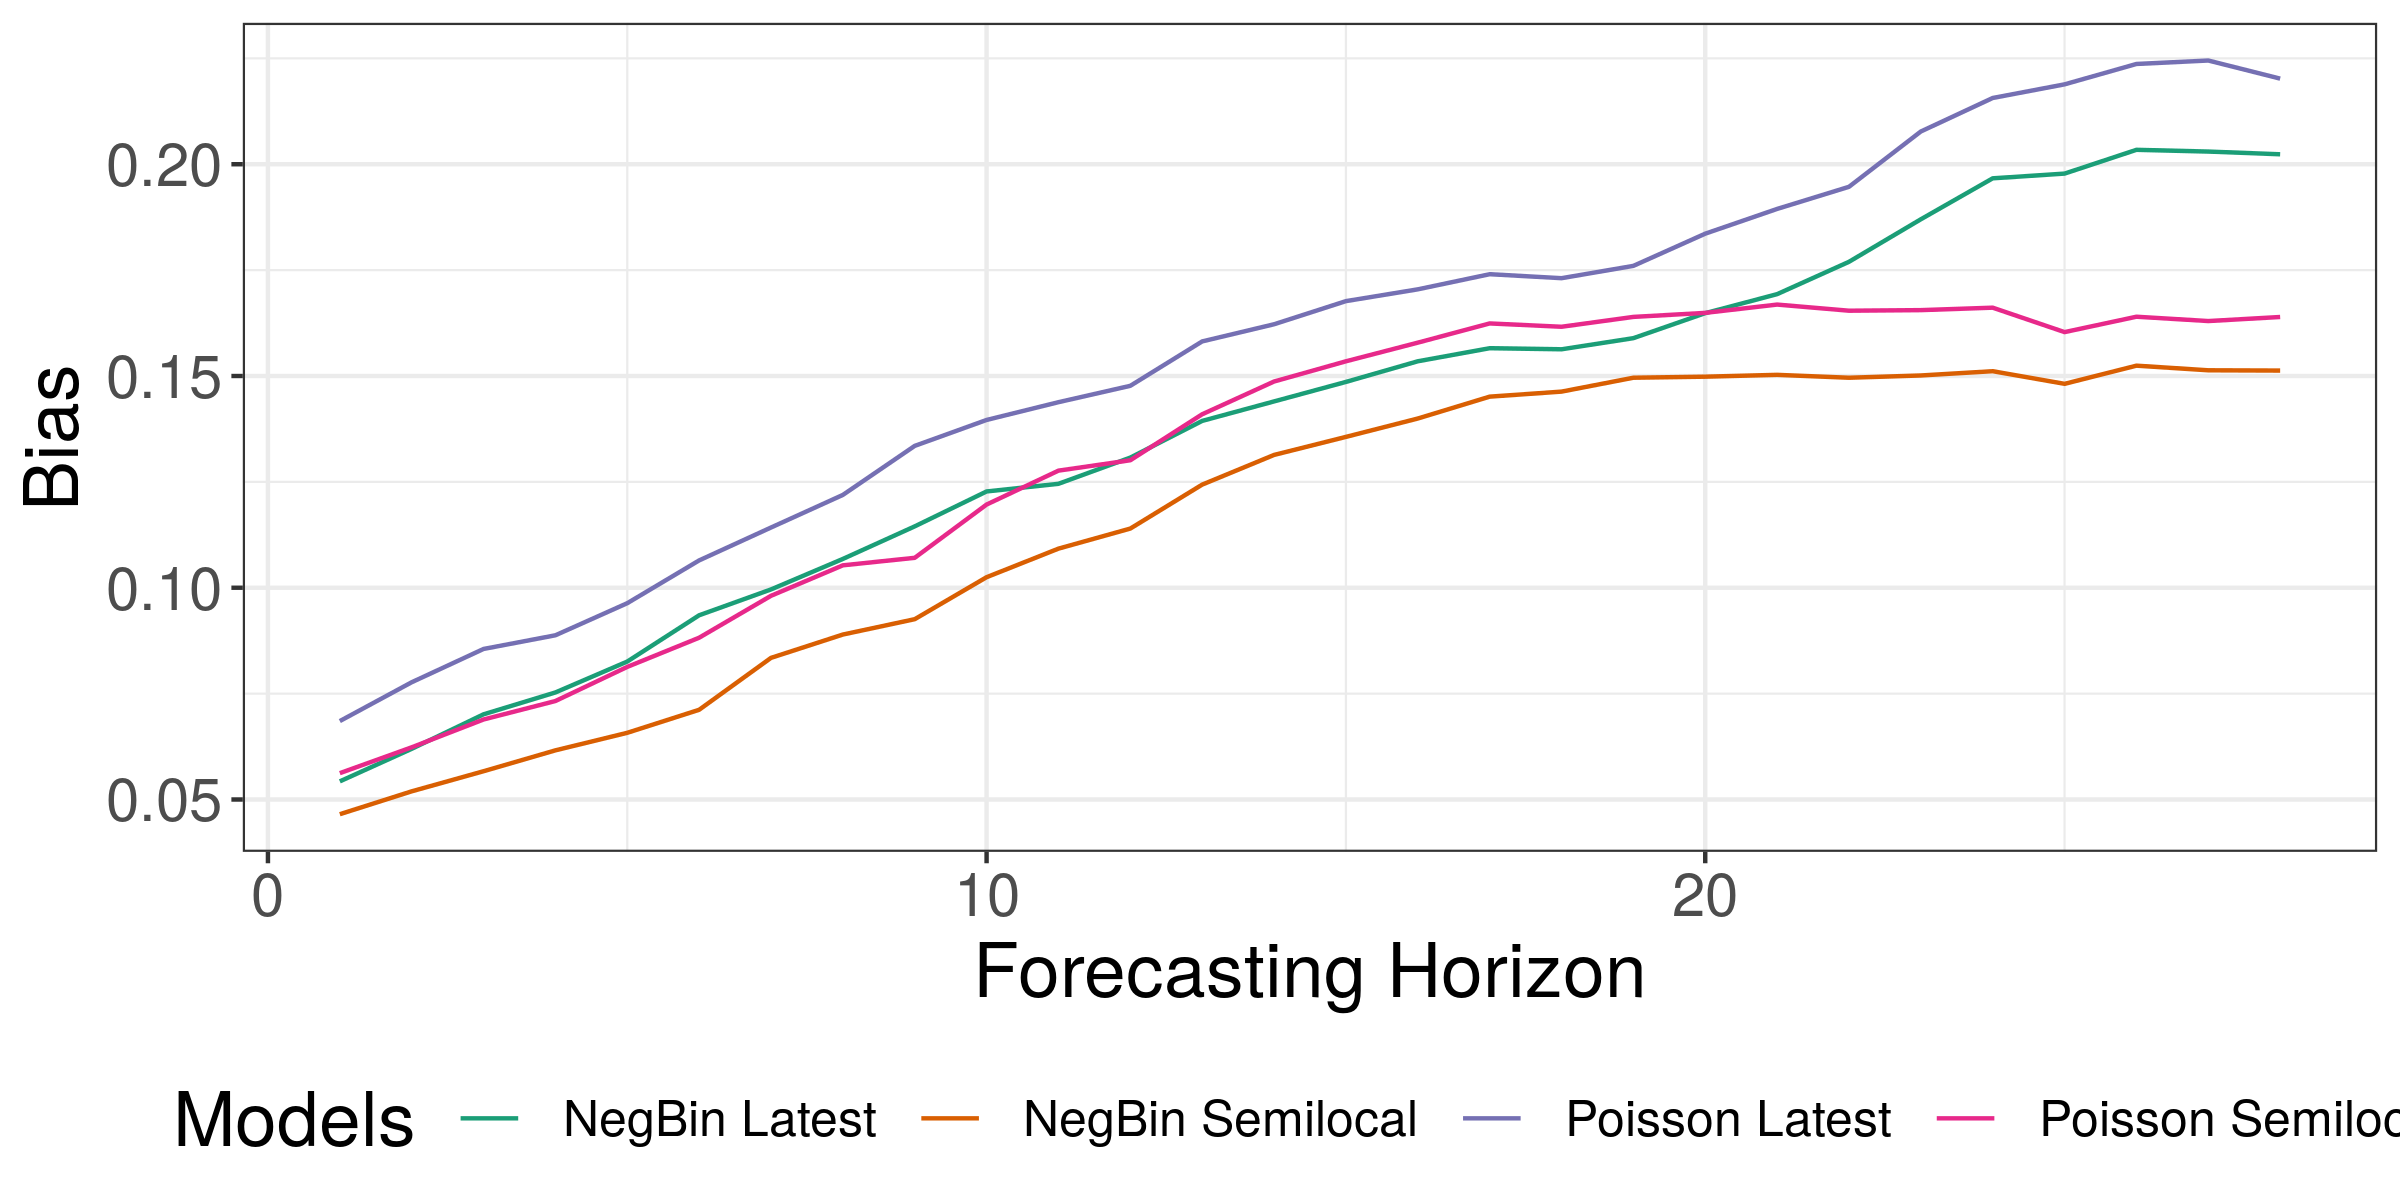
\includegraphics[width=\linewidth]{../output/Butembo_bias.png}  
  \caption{Bias}
  \label{fig:Butembo_scores_3}
\end{subfigure}
\begin{subfigure}{0.5\textwidth}
  \centering
  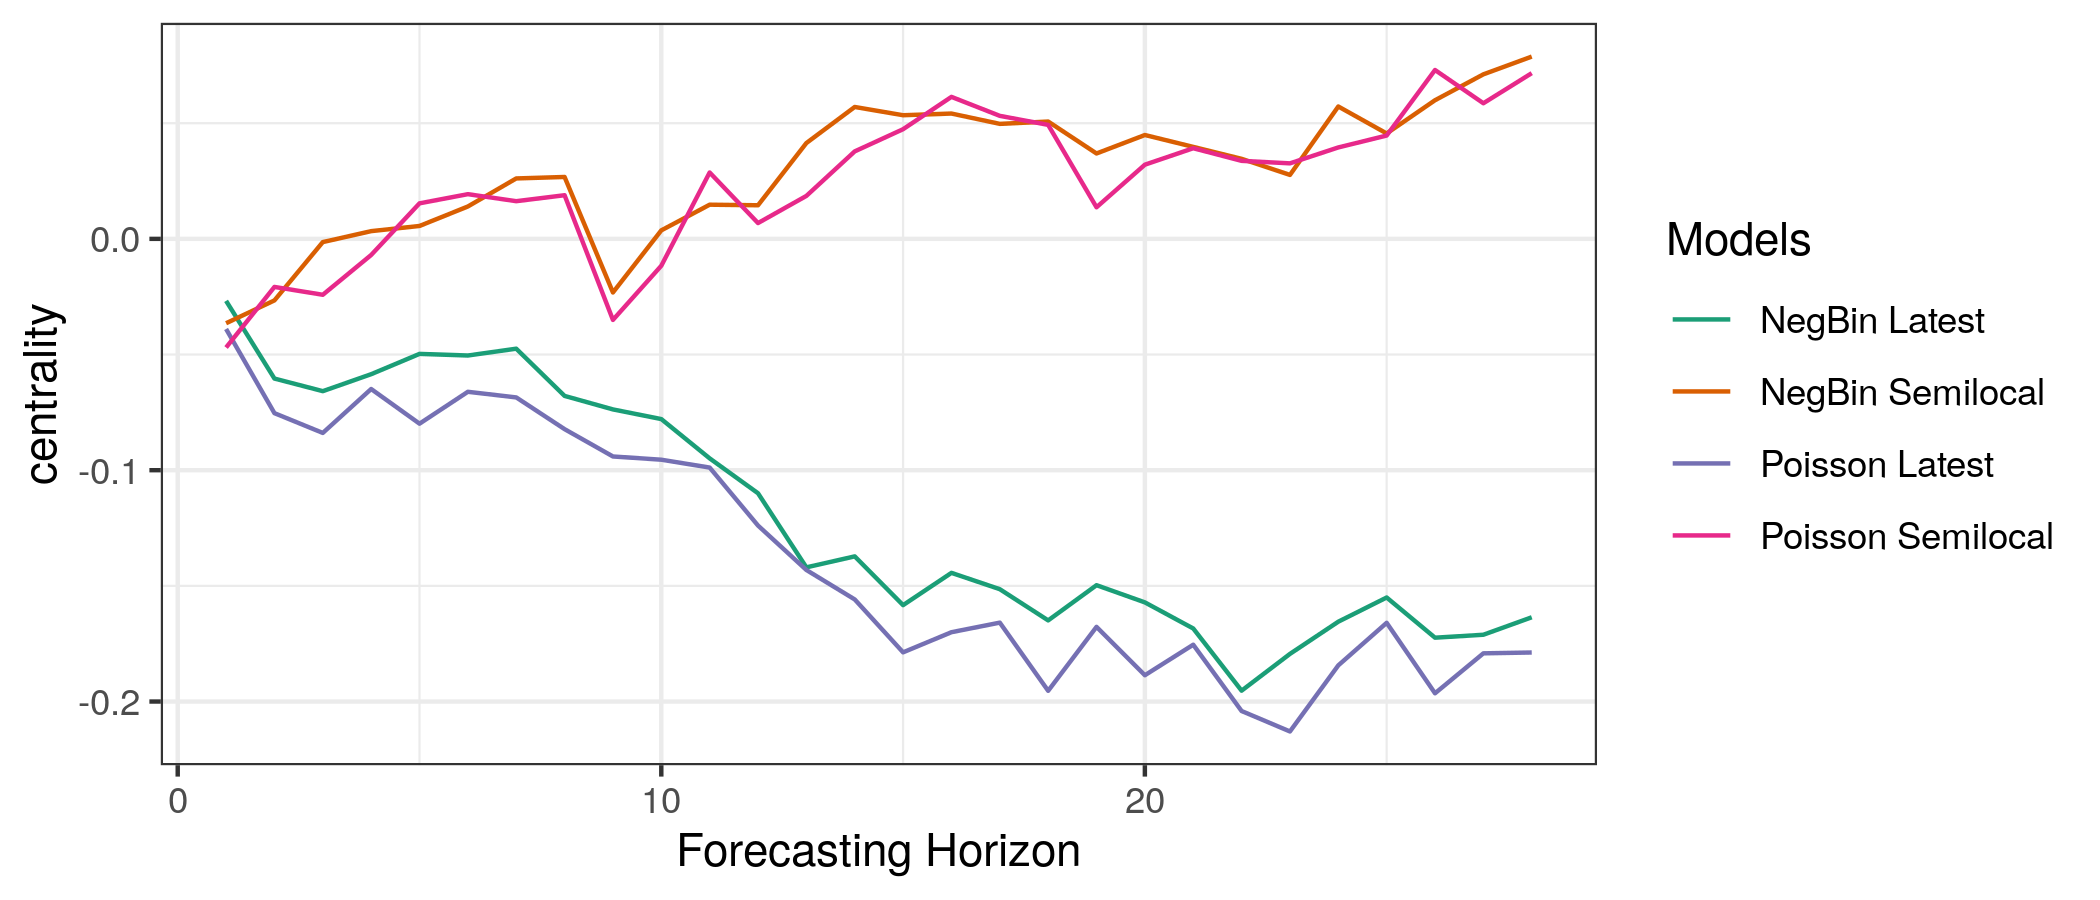
\includegraphics[width=\linewidth]{../output/Butembo_centrality.png}  
  \caption{Centrality of PIT values}
  \label{fig:Butembo_scores_4}
\end{subfigure}
  \caption{Scores for Butembo as a function of the forecasting horizon.}

  \label{fig:nat_scores}
\end{figure}
 \section{ Mabalako }\begin{figure}[H]\begin{subfigure}{\textwidth}  \centering  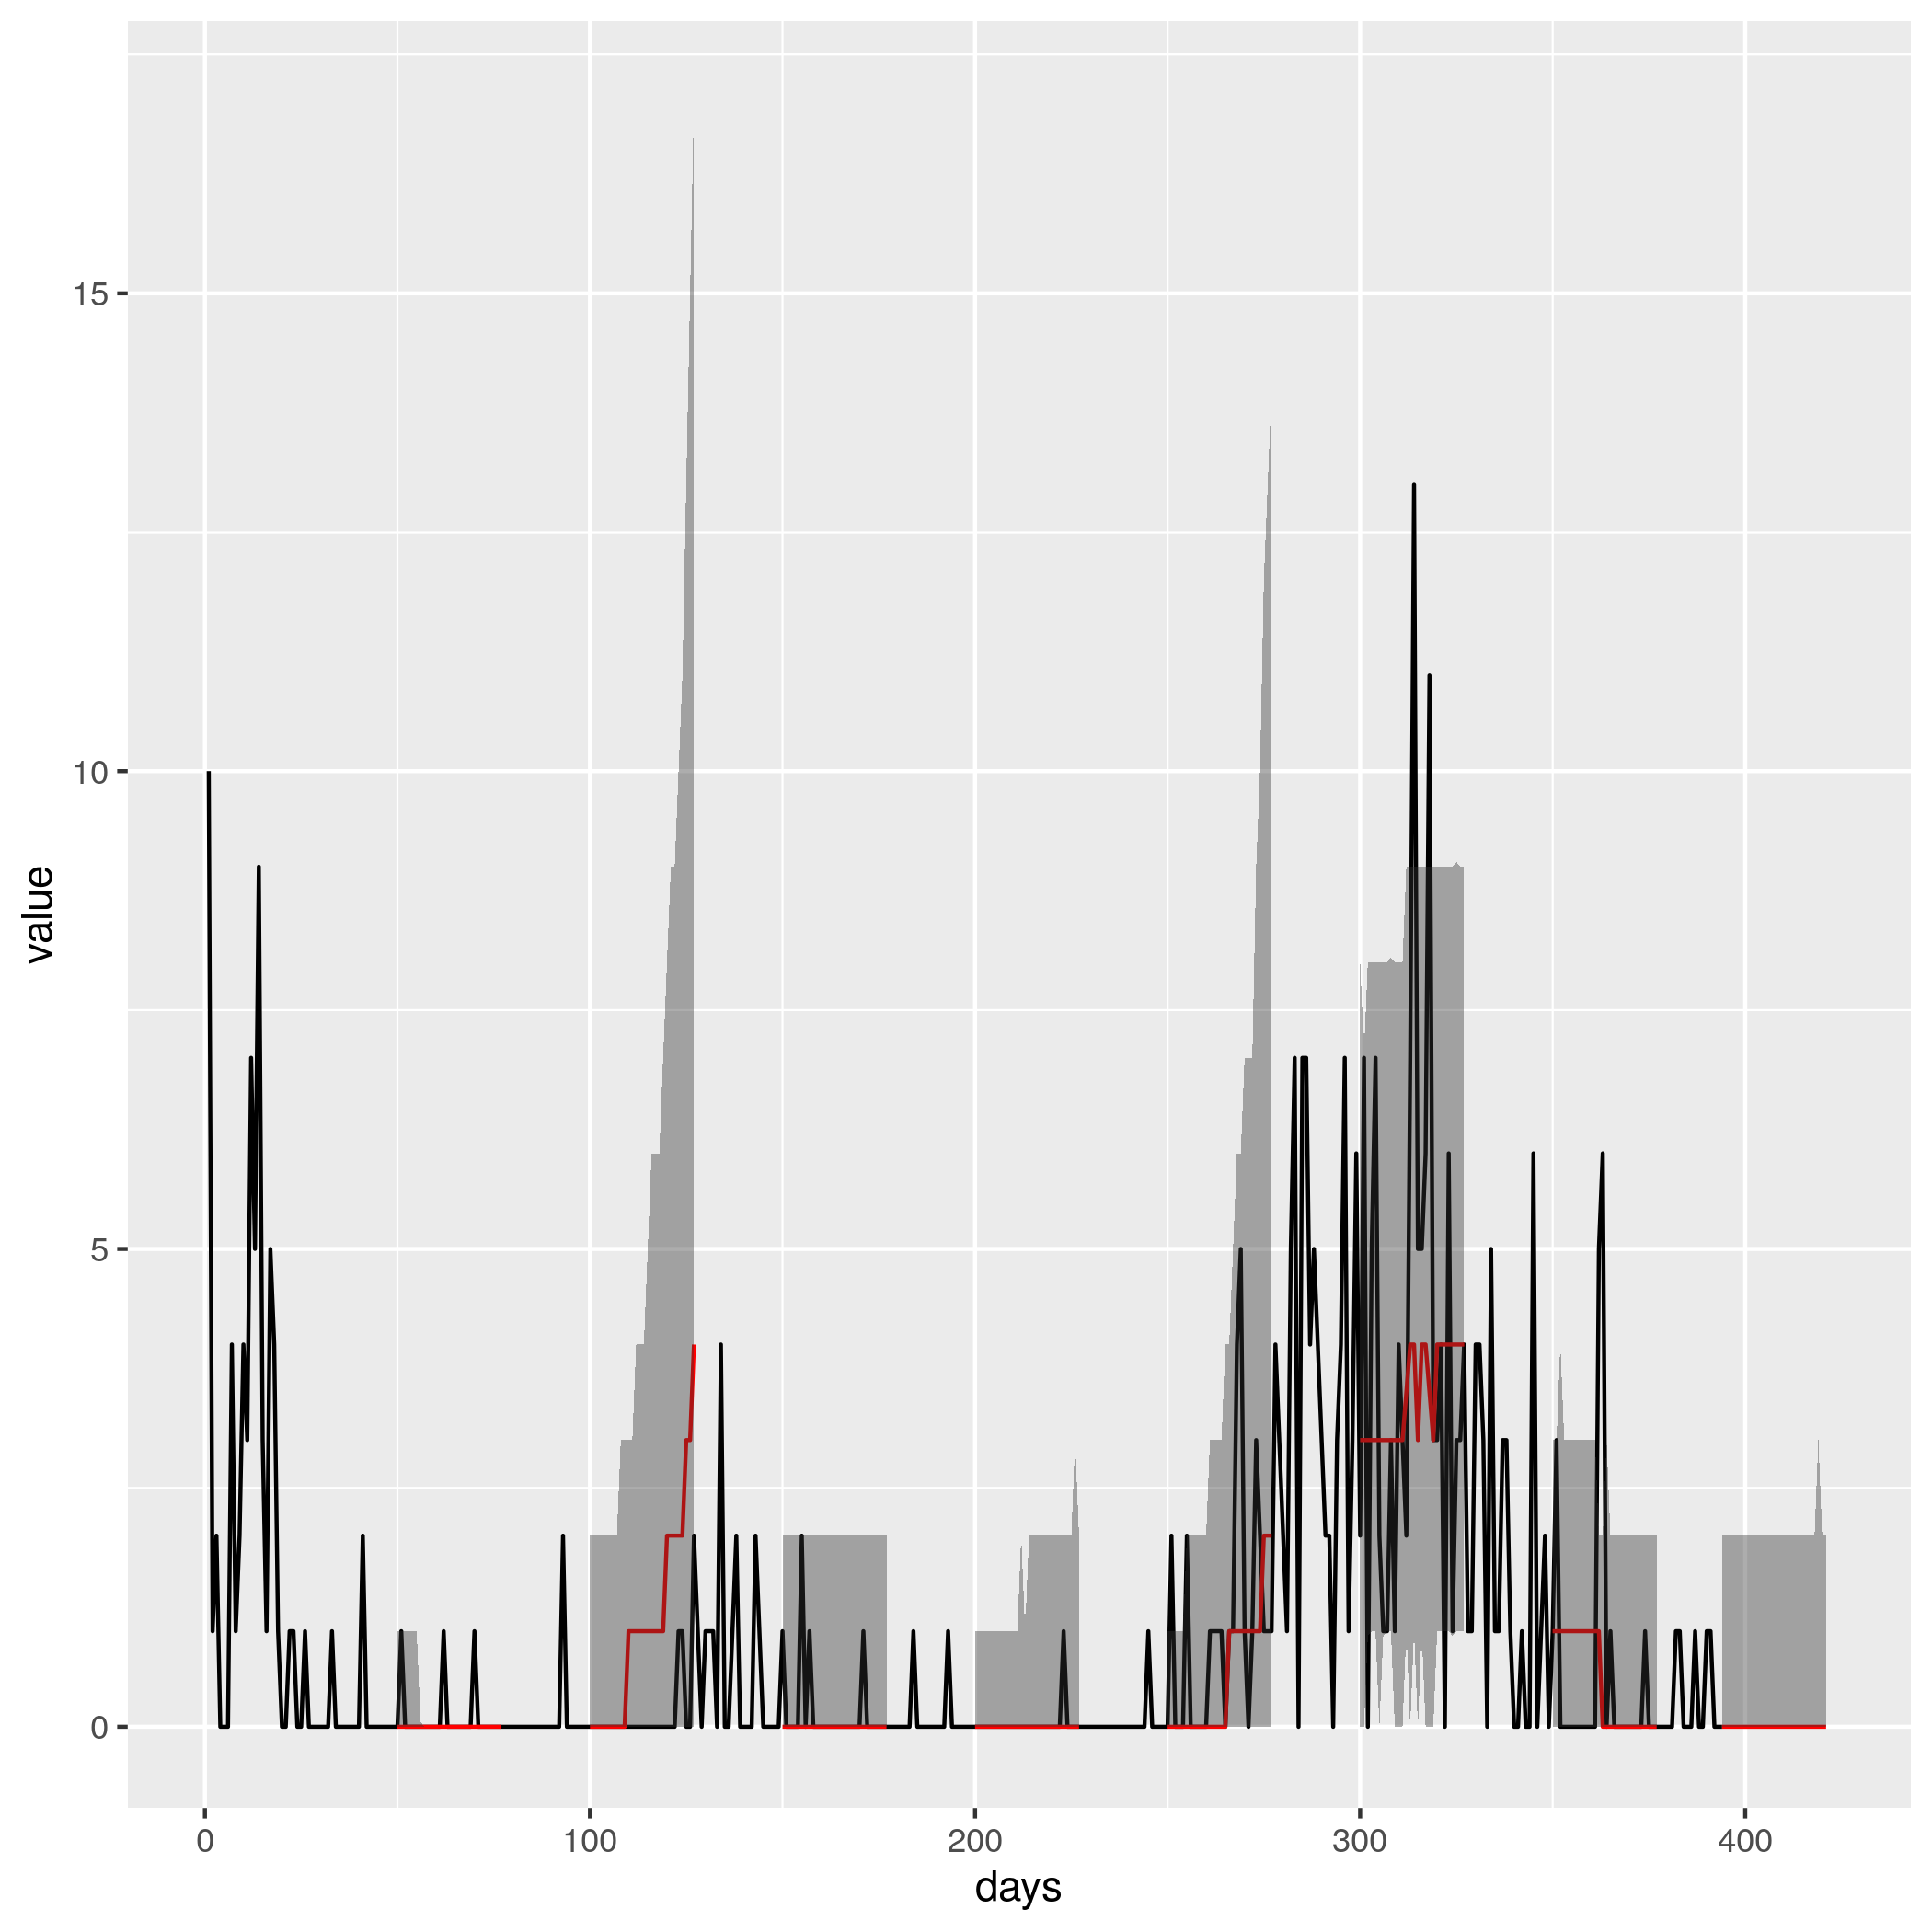
\includegraphics[width=0.9\linewidth, height=7cm]{../output/Mabalako_predictions.png}  \caption{Forecasted and predicted incidence for the best fitting model}\end{subfigure}

\begin{subfigure}{\textwidth}  \centering  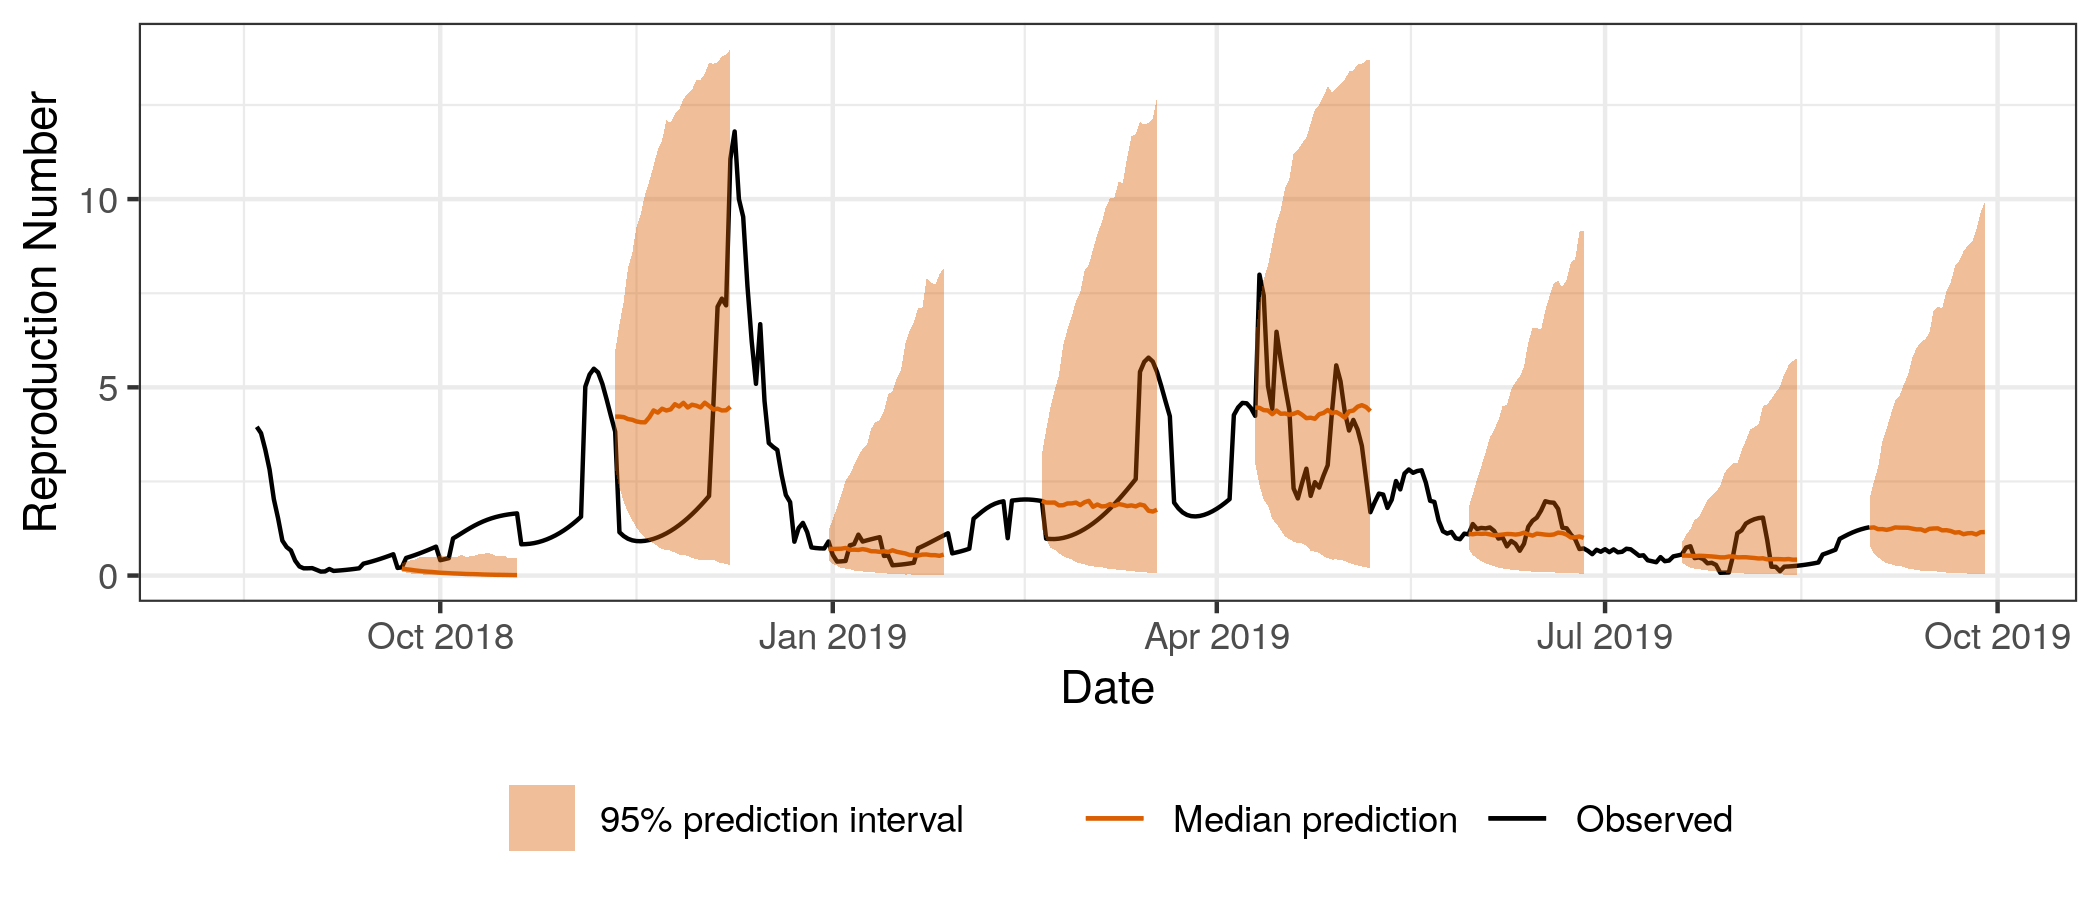
\includegraphics[width=0.9\linewidth, height=7cm]{../output/Mabalako_Rs.png}  \caption{Forecasted and predicted repreoduction numbers for the best fitting model}\end{subfigure}  \caption{Median forecast with 95 \% prediction intervals and observed values for incidence and reproduction number for the best fitting model for Mabalako.}\end{figure}

\begin{figure}[H]
\begin{subfigure}{0.5\textwidth}
  \centering
  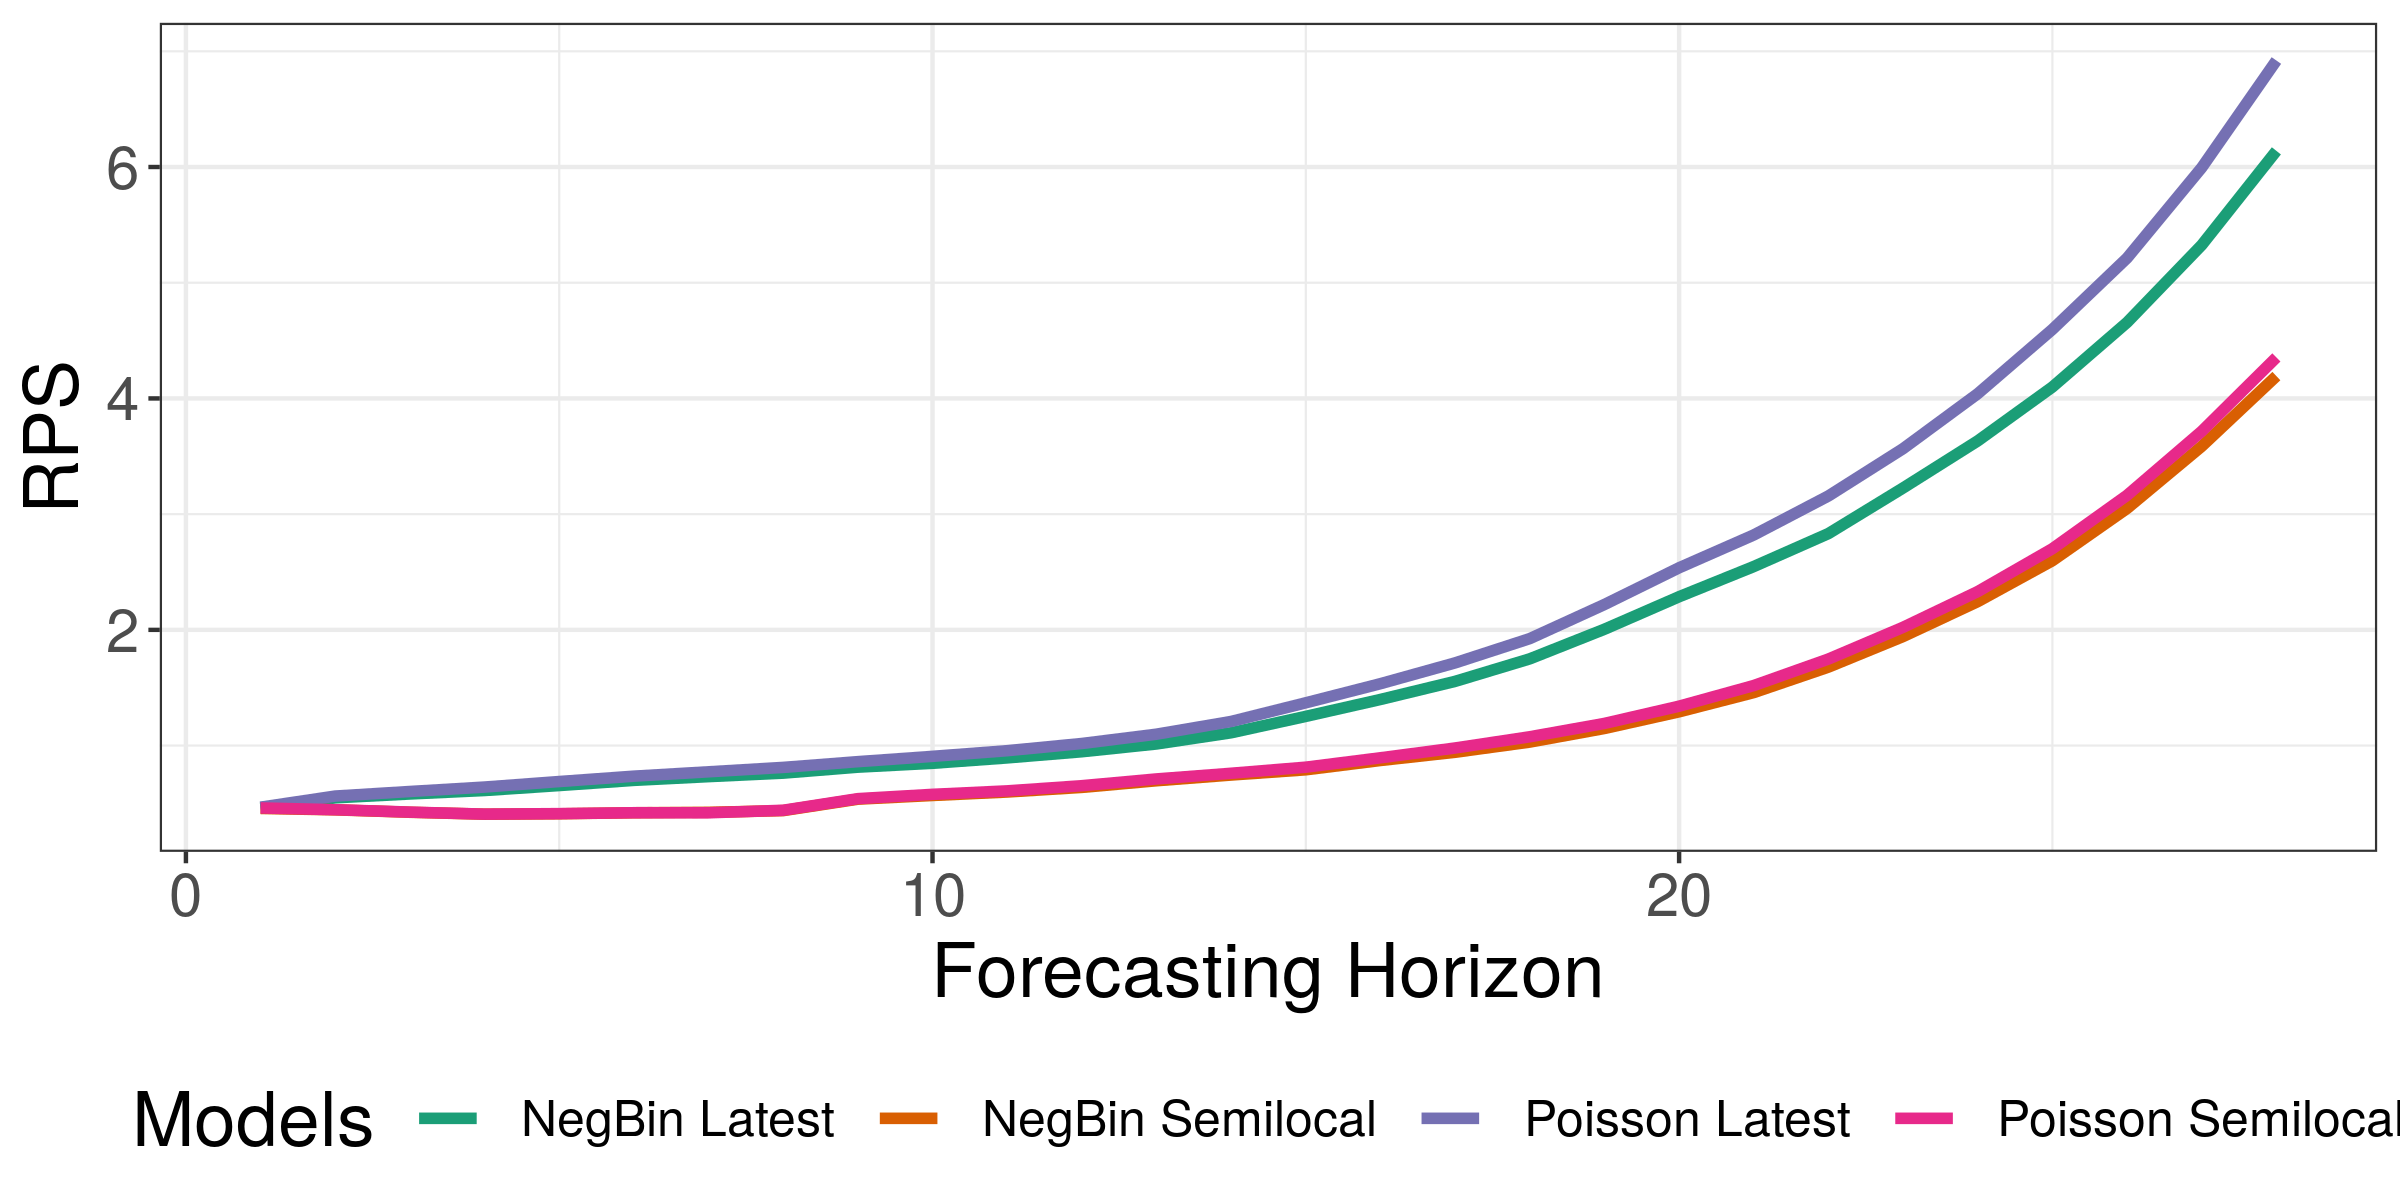
\includegraphics[width=\linewidth]{../output/Mabalako_crps.png}  
  \caption{Contineously Ranked Probability Score}
  \label{Mabalako_scores_1}
\end{subfigure}
\begin{subfigure}{0.5\textwidth}
  \centering
  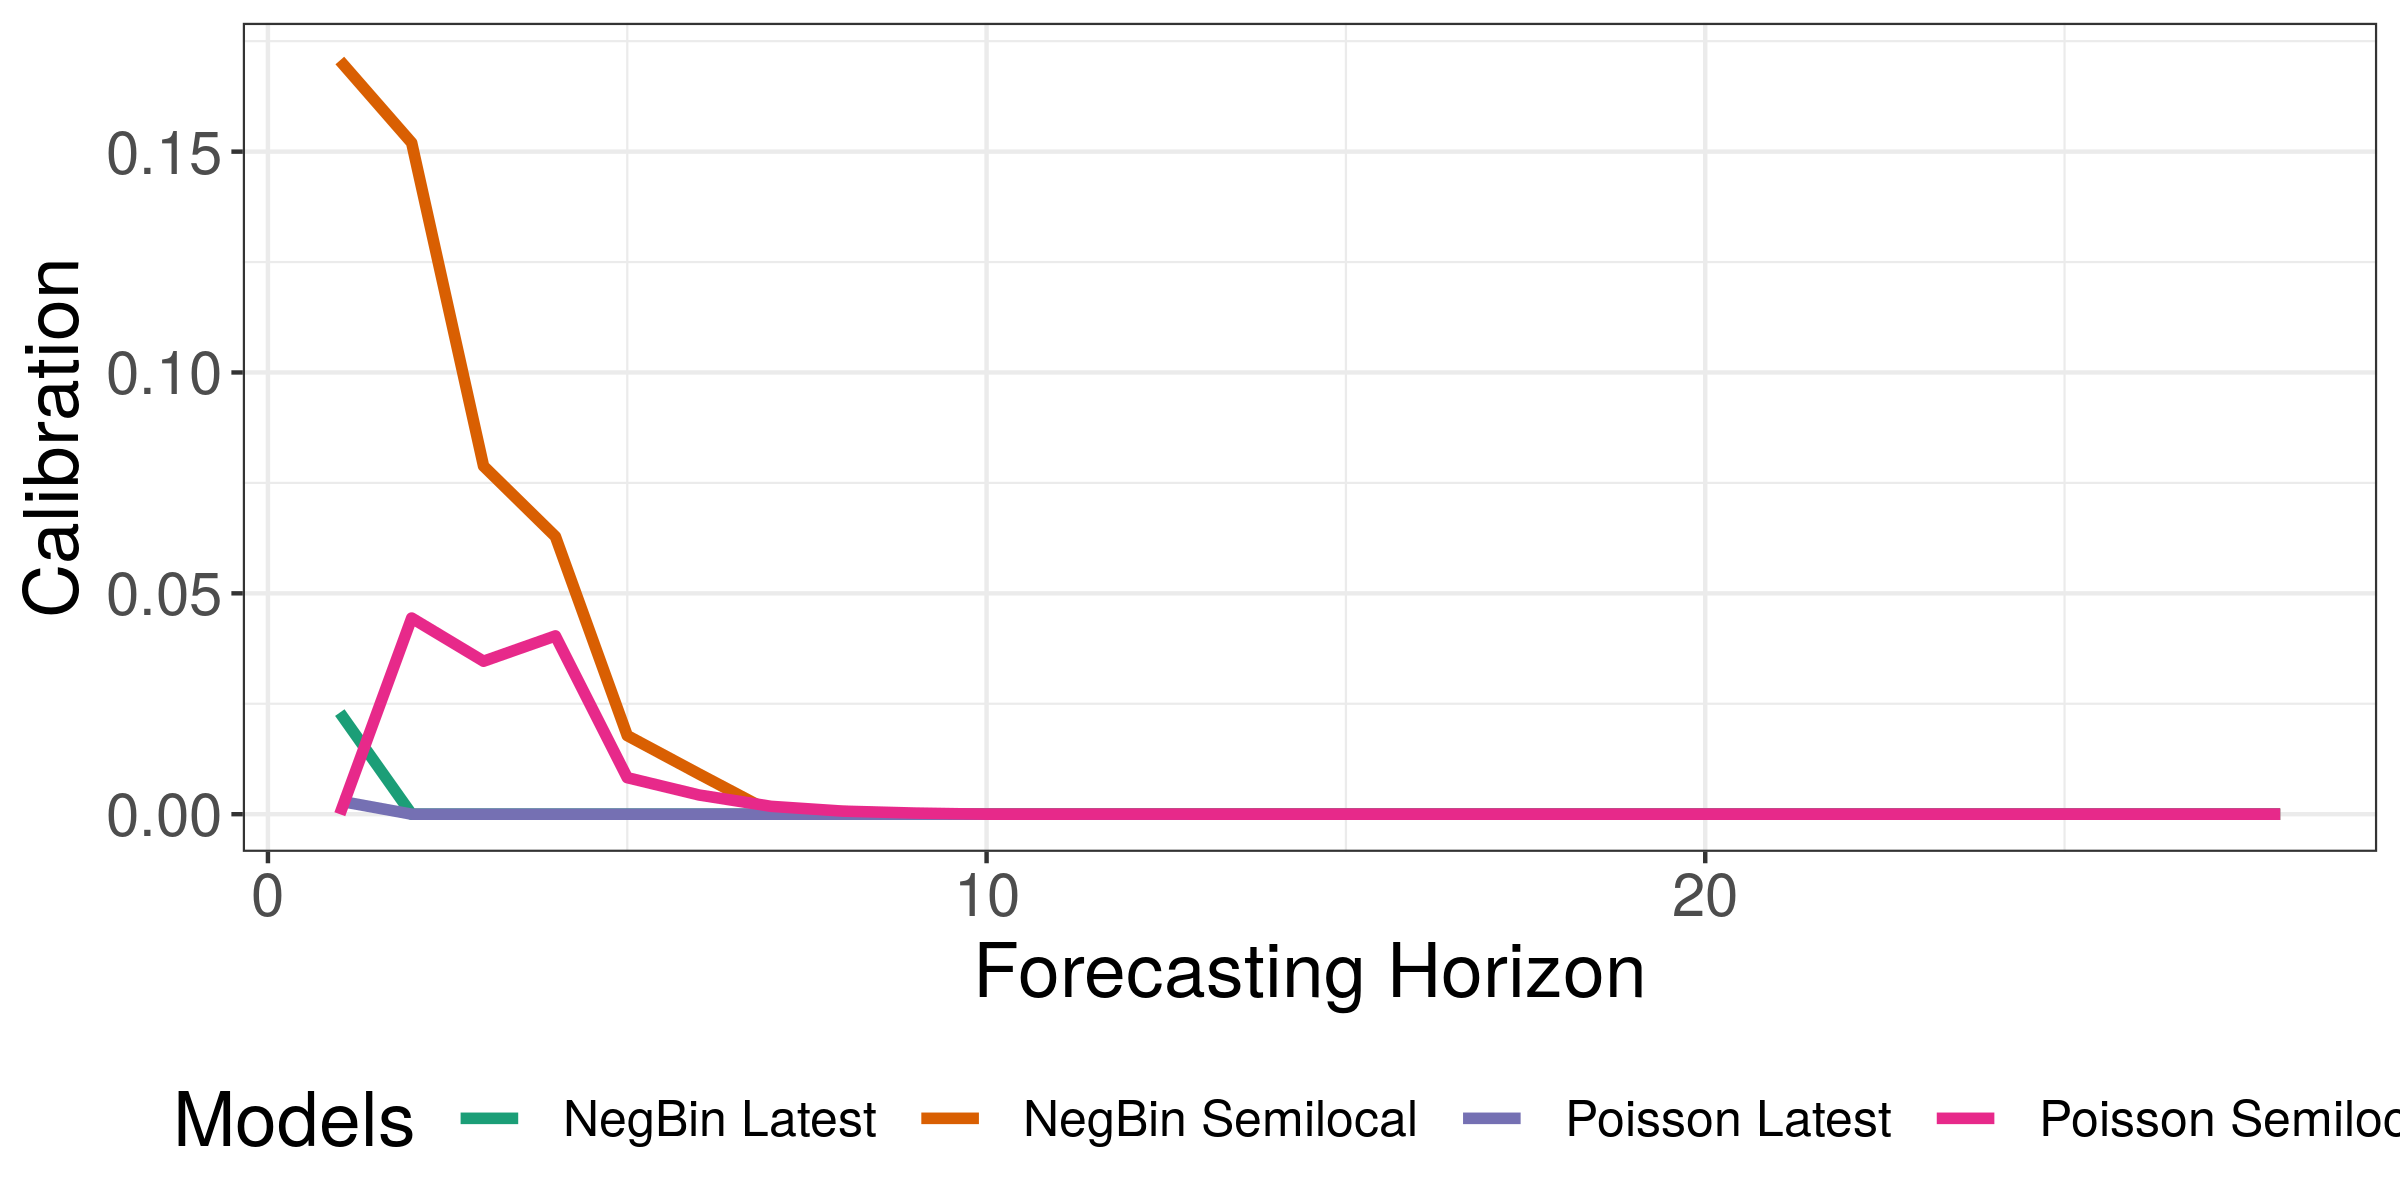
\includegraphics[width=\linewidth]{../output/Mabalako_calibration.png}  
  \caption{Calibration p-value}
  \label{Mabalako_scores_2}
\end{subfigure}

\begin{subfigure}{0.5\textwidth}
  \centering
  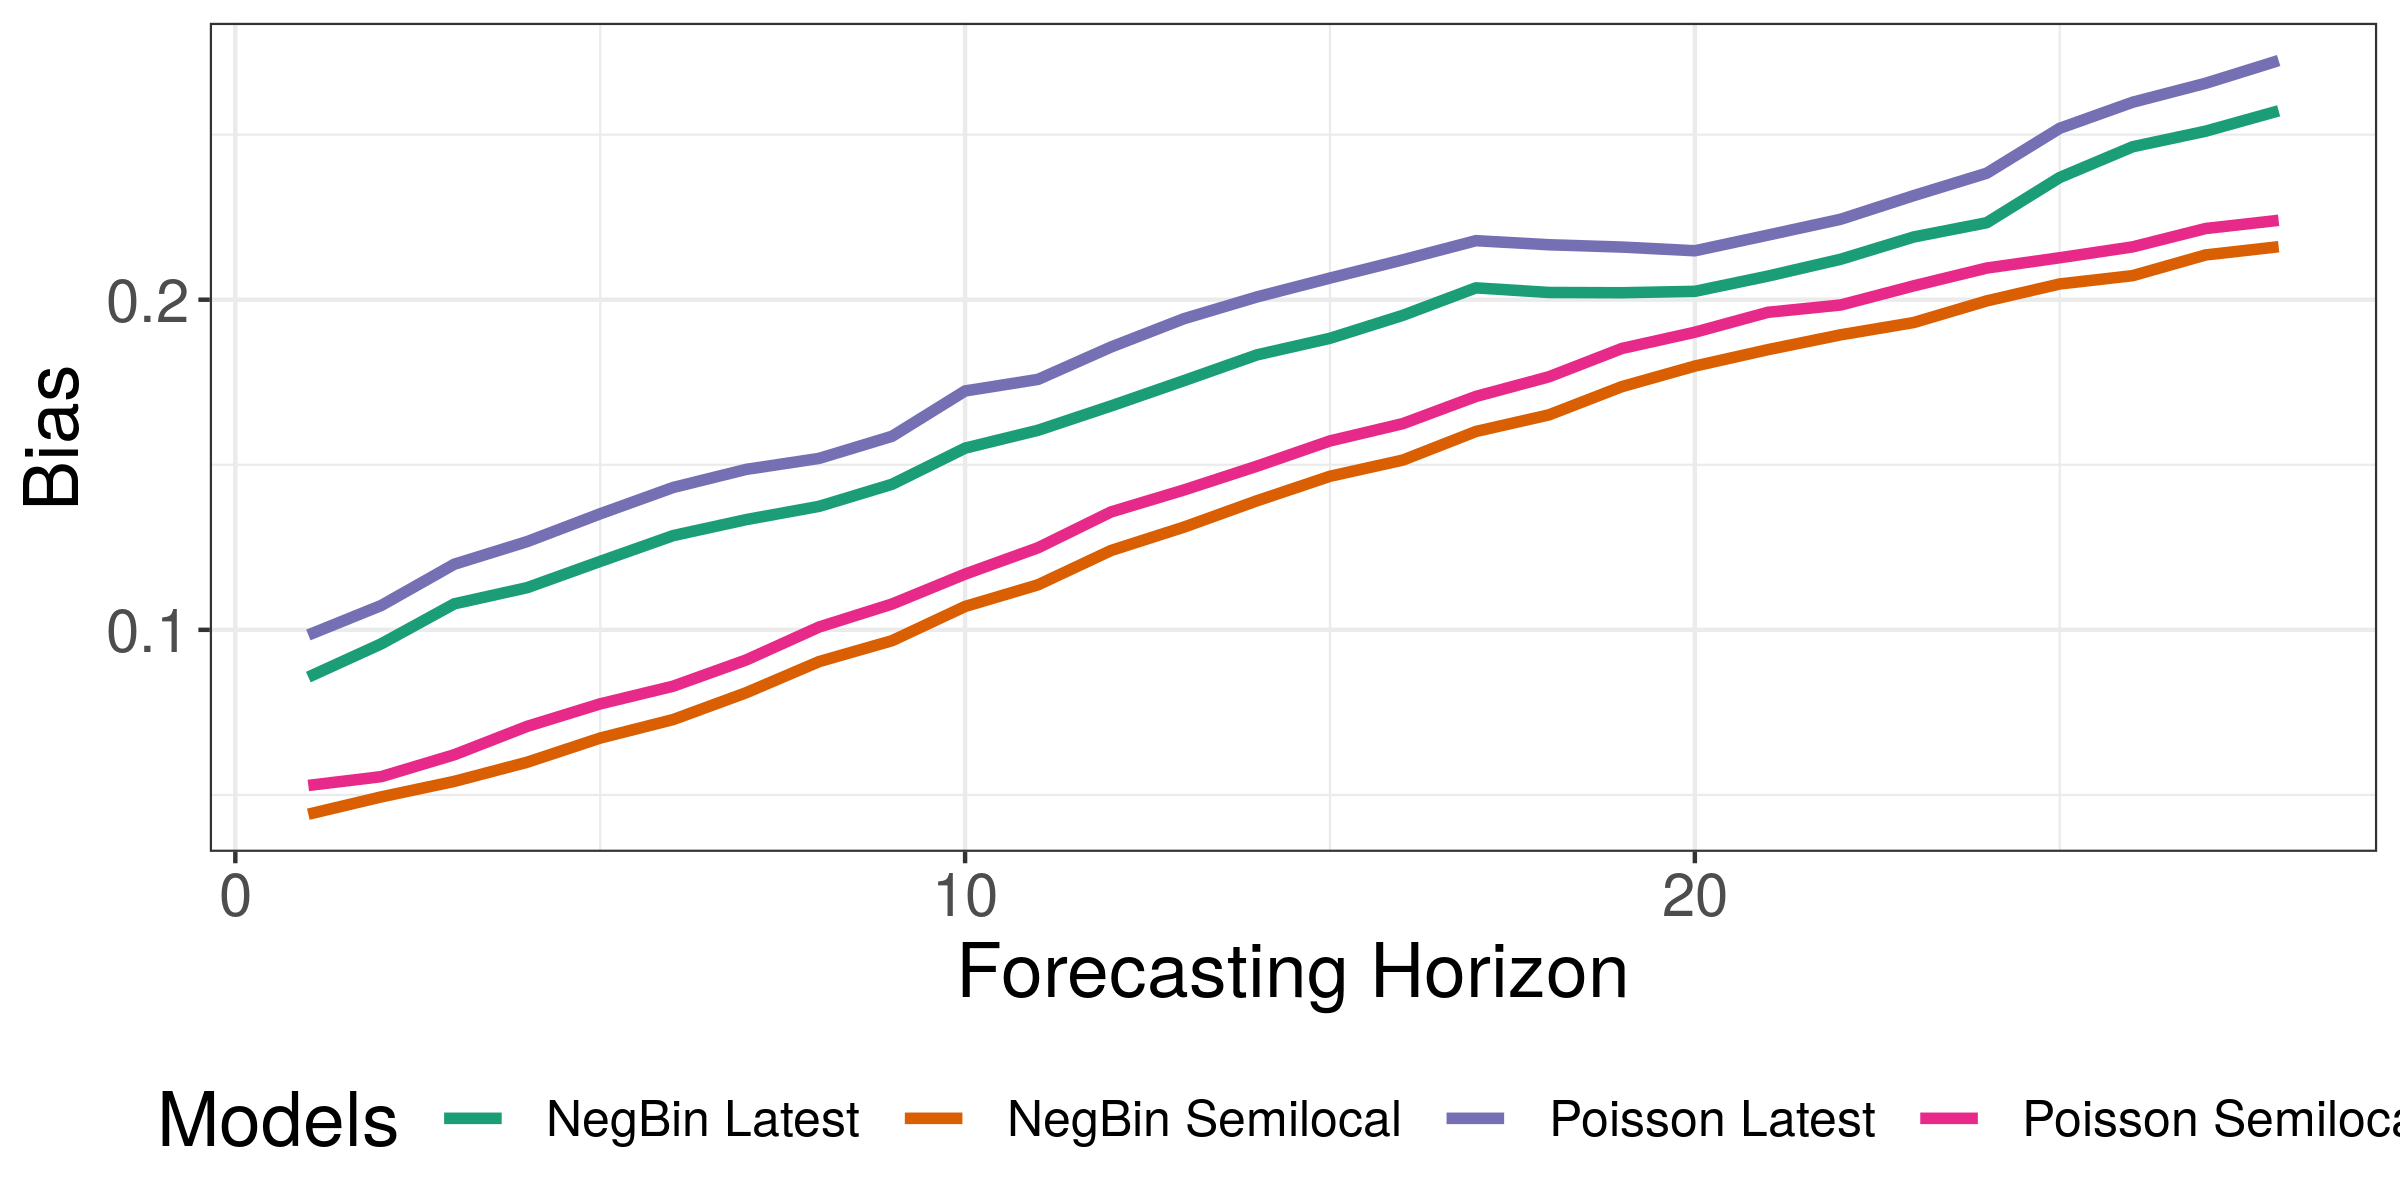
\includegraphics[width=\linewidth]{../output/Mabalako_bias.png}  
  \caption{Bias}
  \label{fig:Mabalako_scores_3}
\end{subfigure}
\begin{subfigure}{0.5\textwidth}
  \centering
  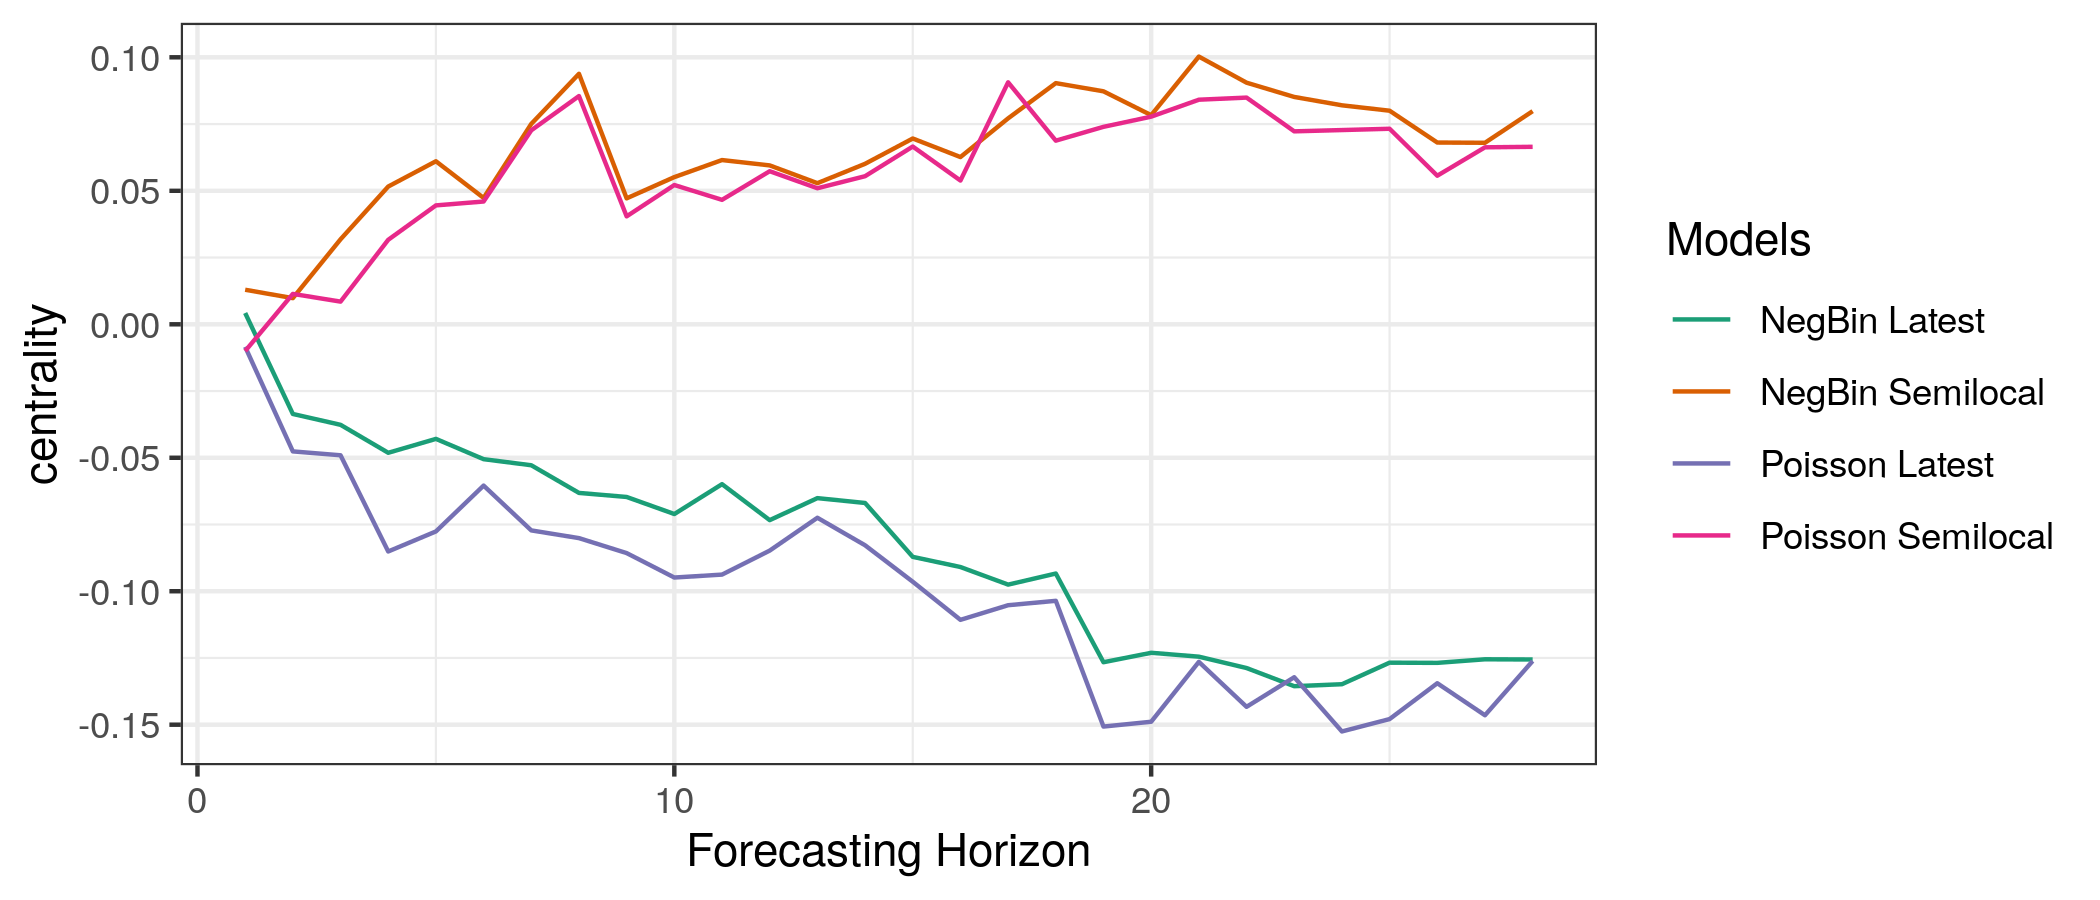
\includegraphics[width=\linewidth]{../output/Mabalako_centrality.png}  
  \caption{Centrality of PIT values}
  \label{fig:Mabalako_scores_4}
\end{subfigure}
  \caption{Scores for Mabalako as a function of the forecasting horizon.}

  \label{fig:nat_scores}
\end{figure}
 \section{ Tchomia }\begin{figure}[H]\begin{subfigure}{\textwidth}  \centering  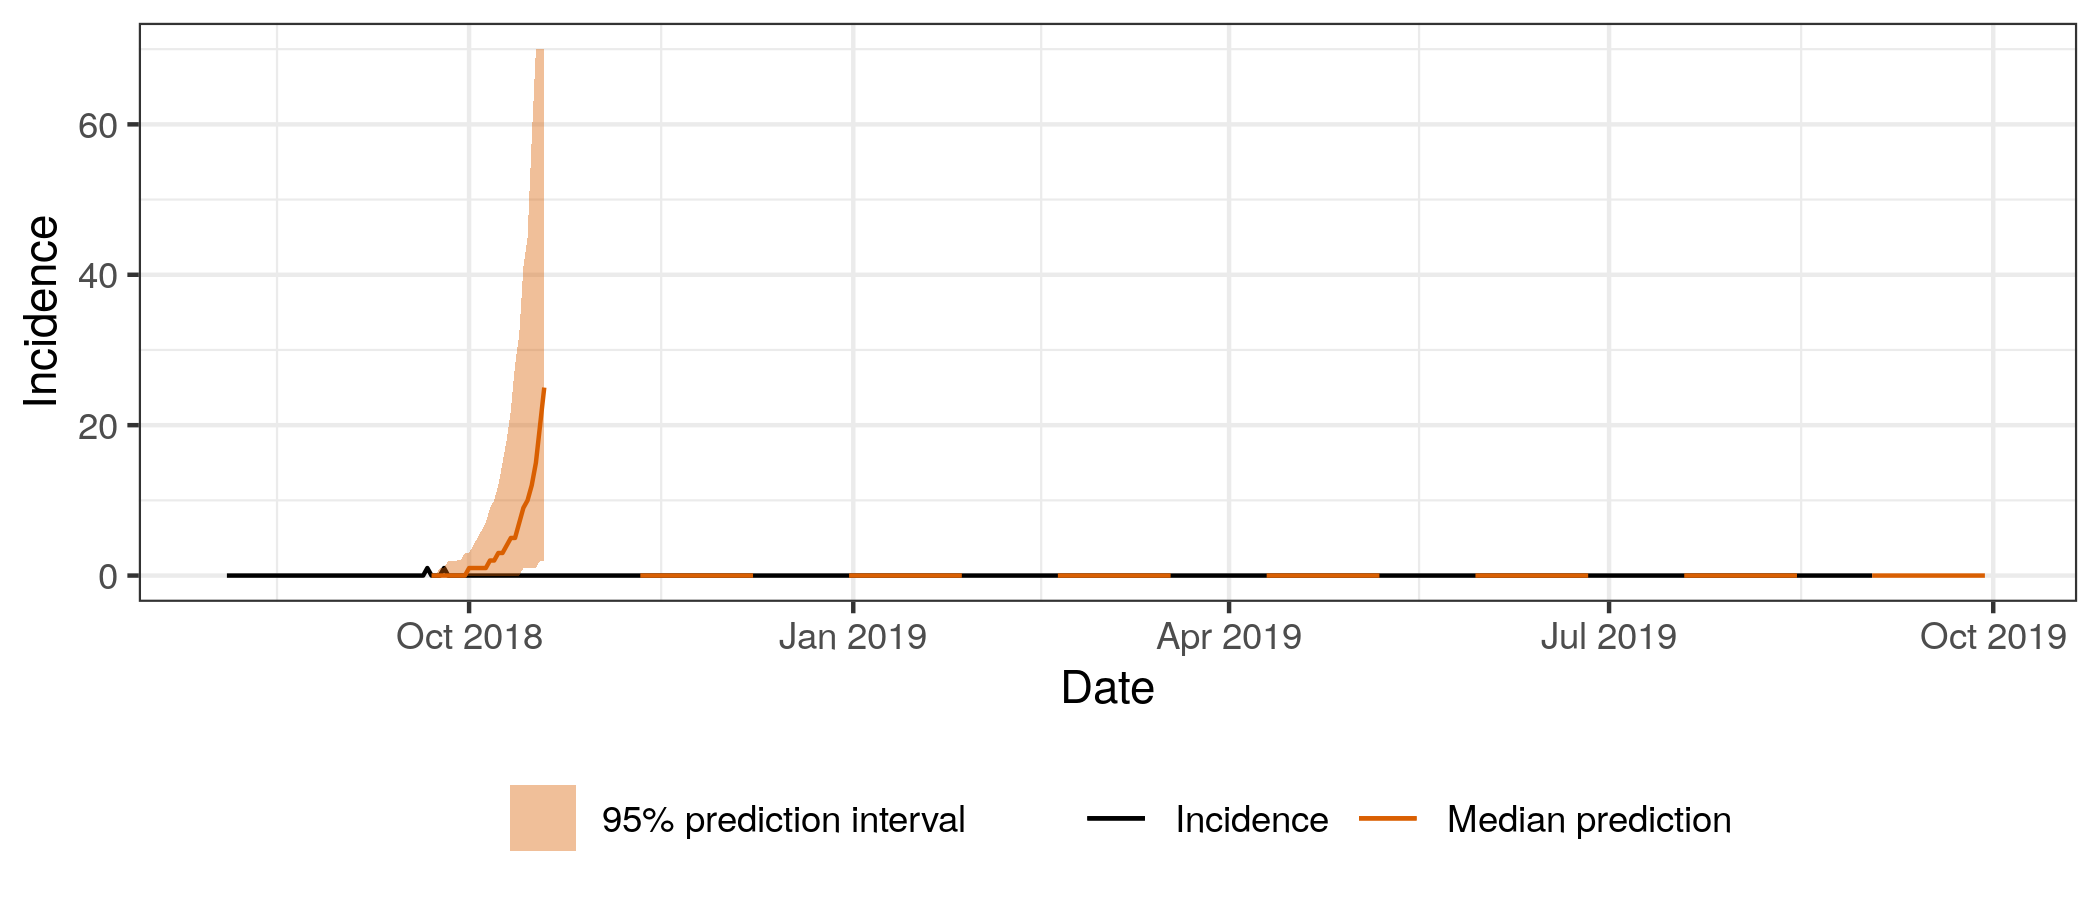
\includegraphics[width=0.9\linewidth, height=7cm]{../output/Tchomia_predictions.png}  \caption{Forecasted and predicted incidence for the best fitting model}\end{subfigure}

\begin{subfigure}{\textwidth}  \centering  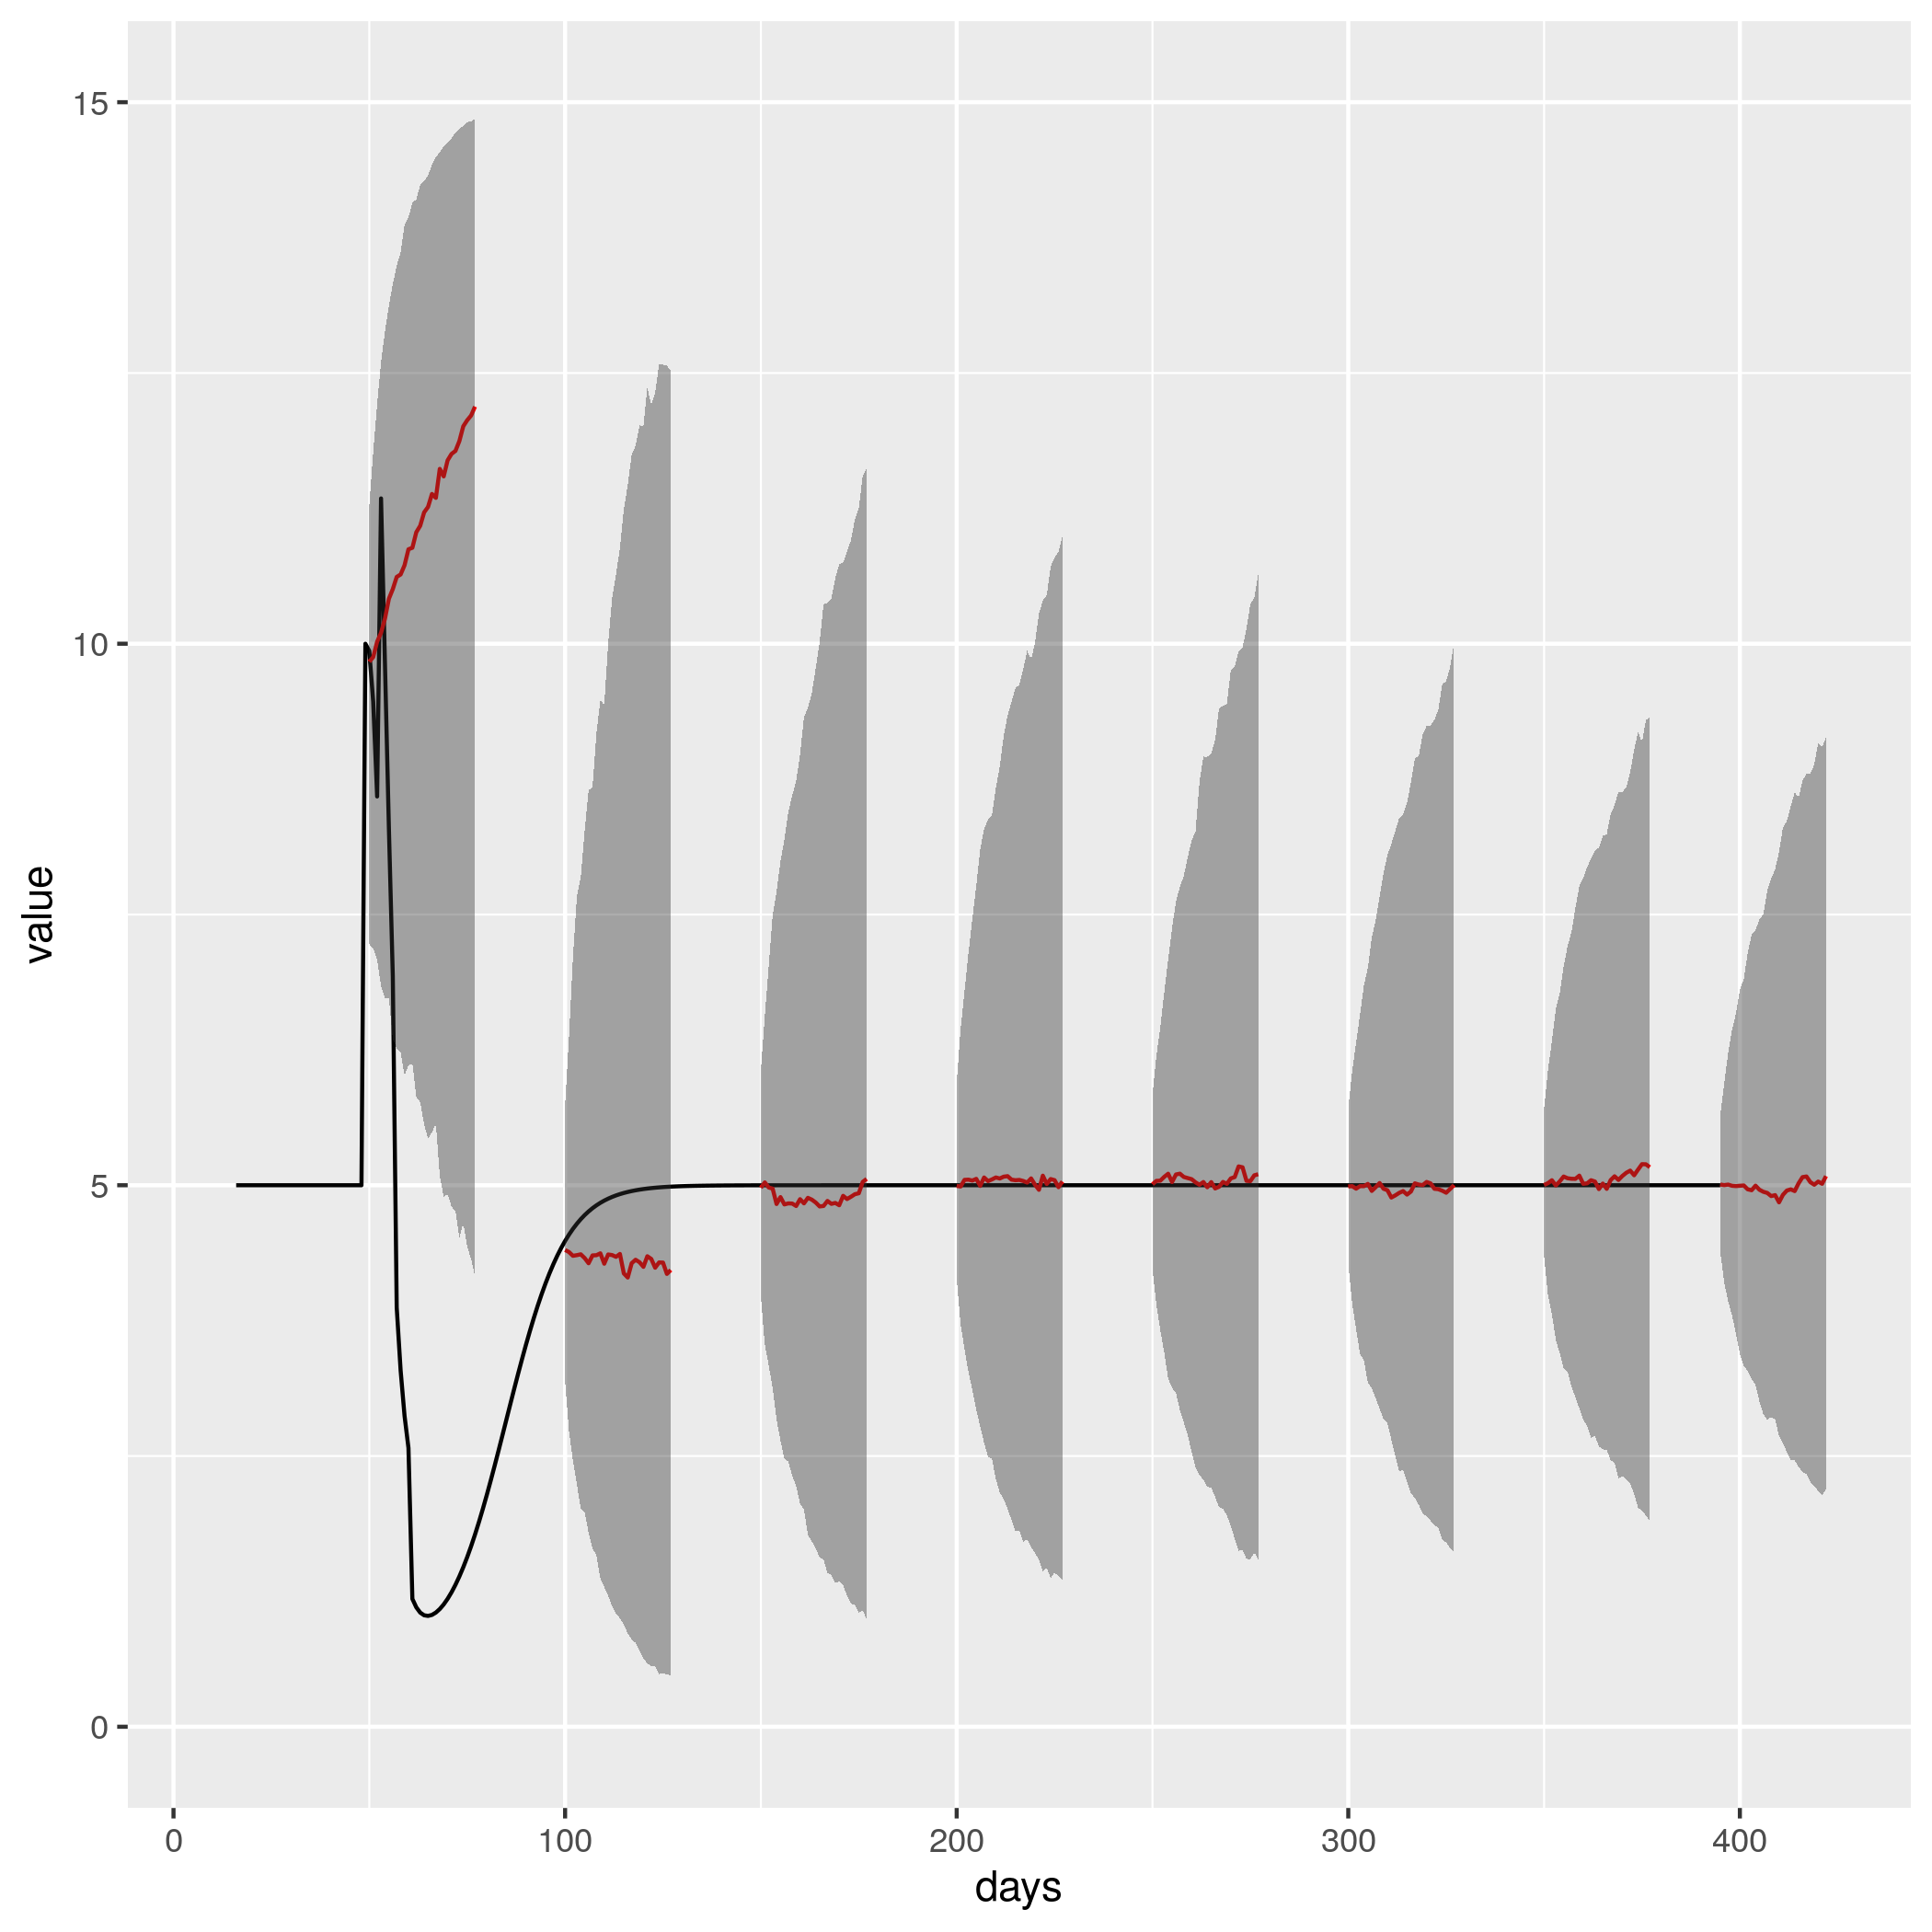
\includegraphics[width=0.9\linewidth, height=7cm]{../output/Tchomia_Rs.png}  \caption{Forecasted and predicted repreoduction numbers for the best fitting model}\end{subfigure}  \caption{Median forecast with 95 \% prediction intervals and observed values for incidence and reproduction number for the best fitting model for Tchomia.}\end{figure}

\begin{figure}[H]
\begin{subfigure}{0.5\textwidth}
  \centering
  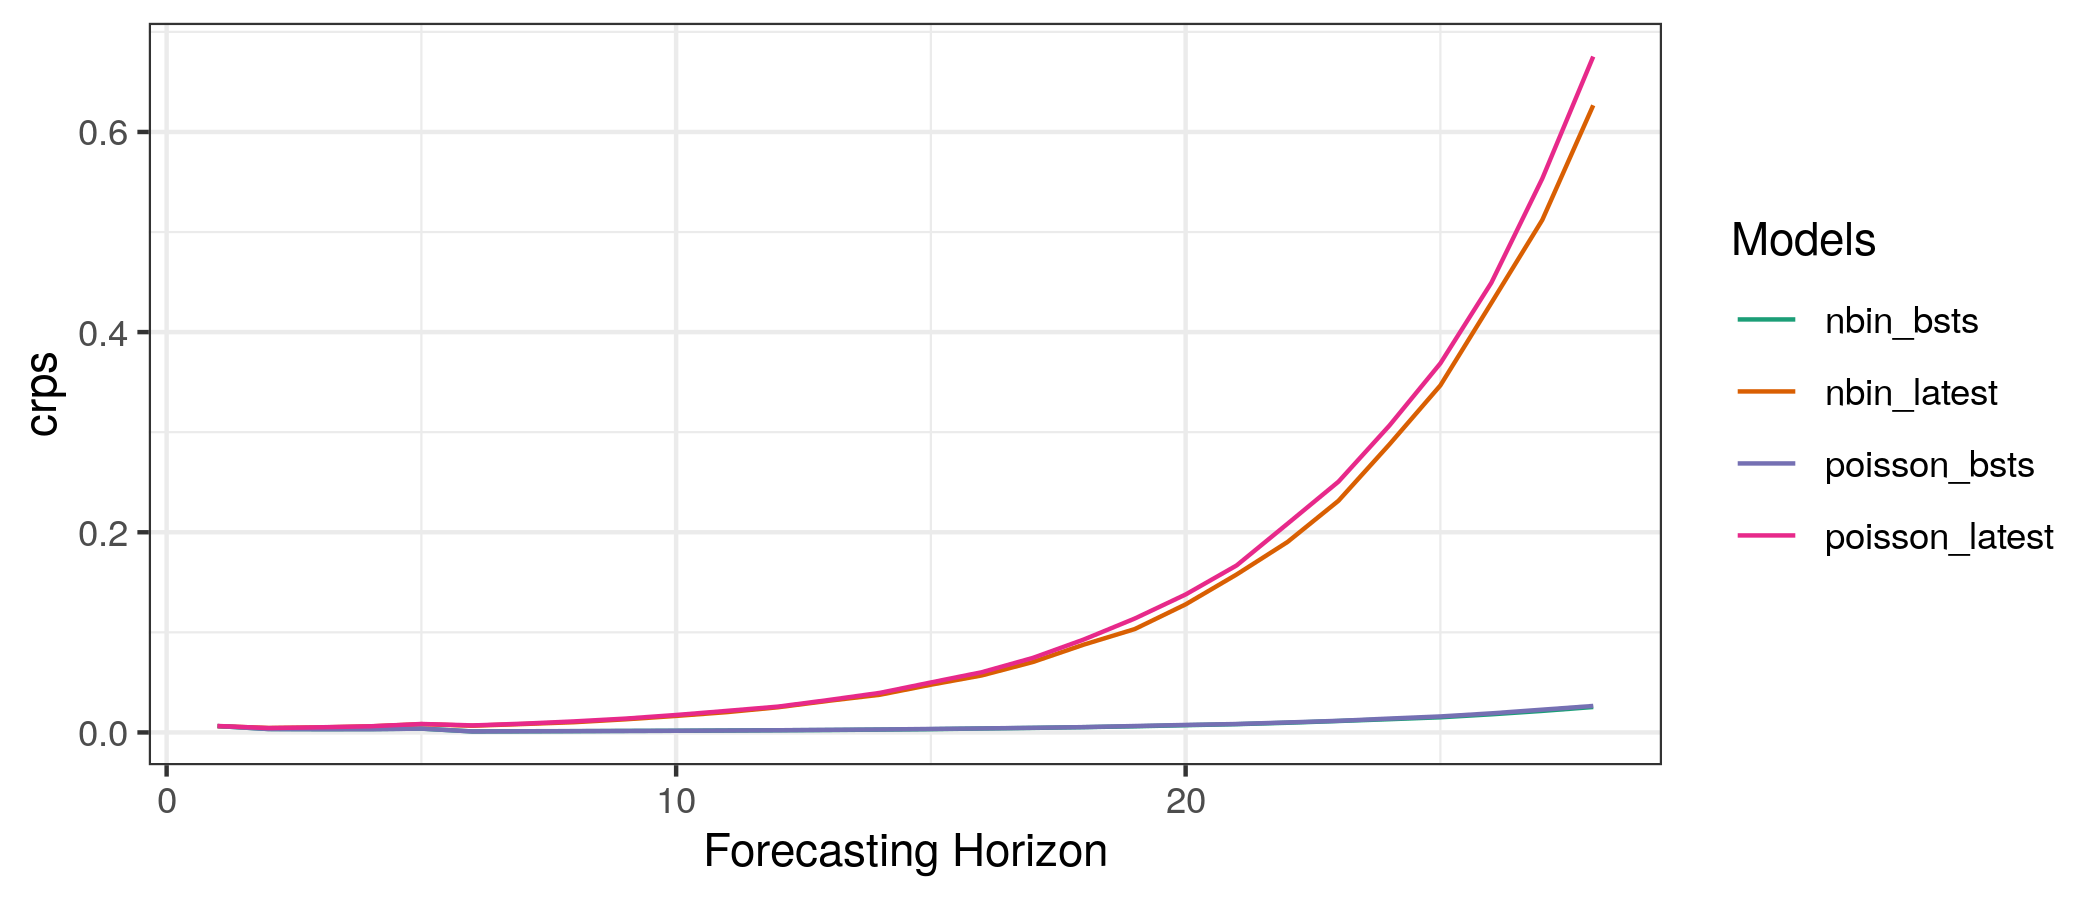
\includegraphics[width=\linewidth]{../output/Tchomia_crps.png}  
  \caption{Contineously Ranked Probability Score}
  \label{Tchomia_scores_1}
\end{subfigure}
\begin{subfigure}{0.5\textwidth}
  \centering
  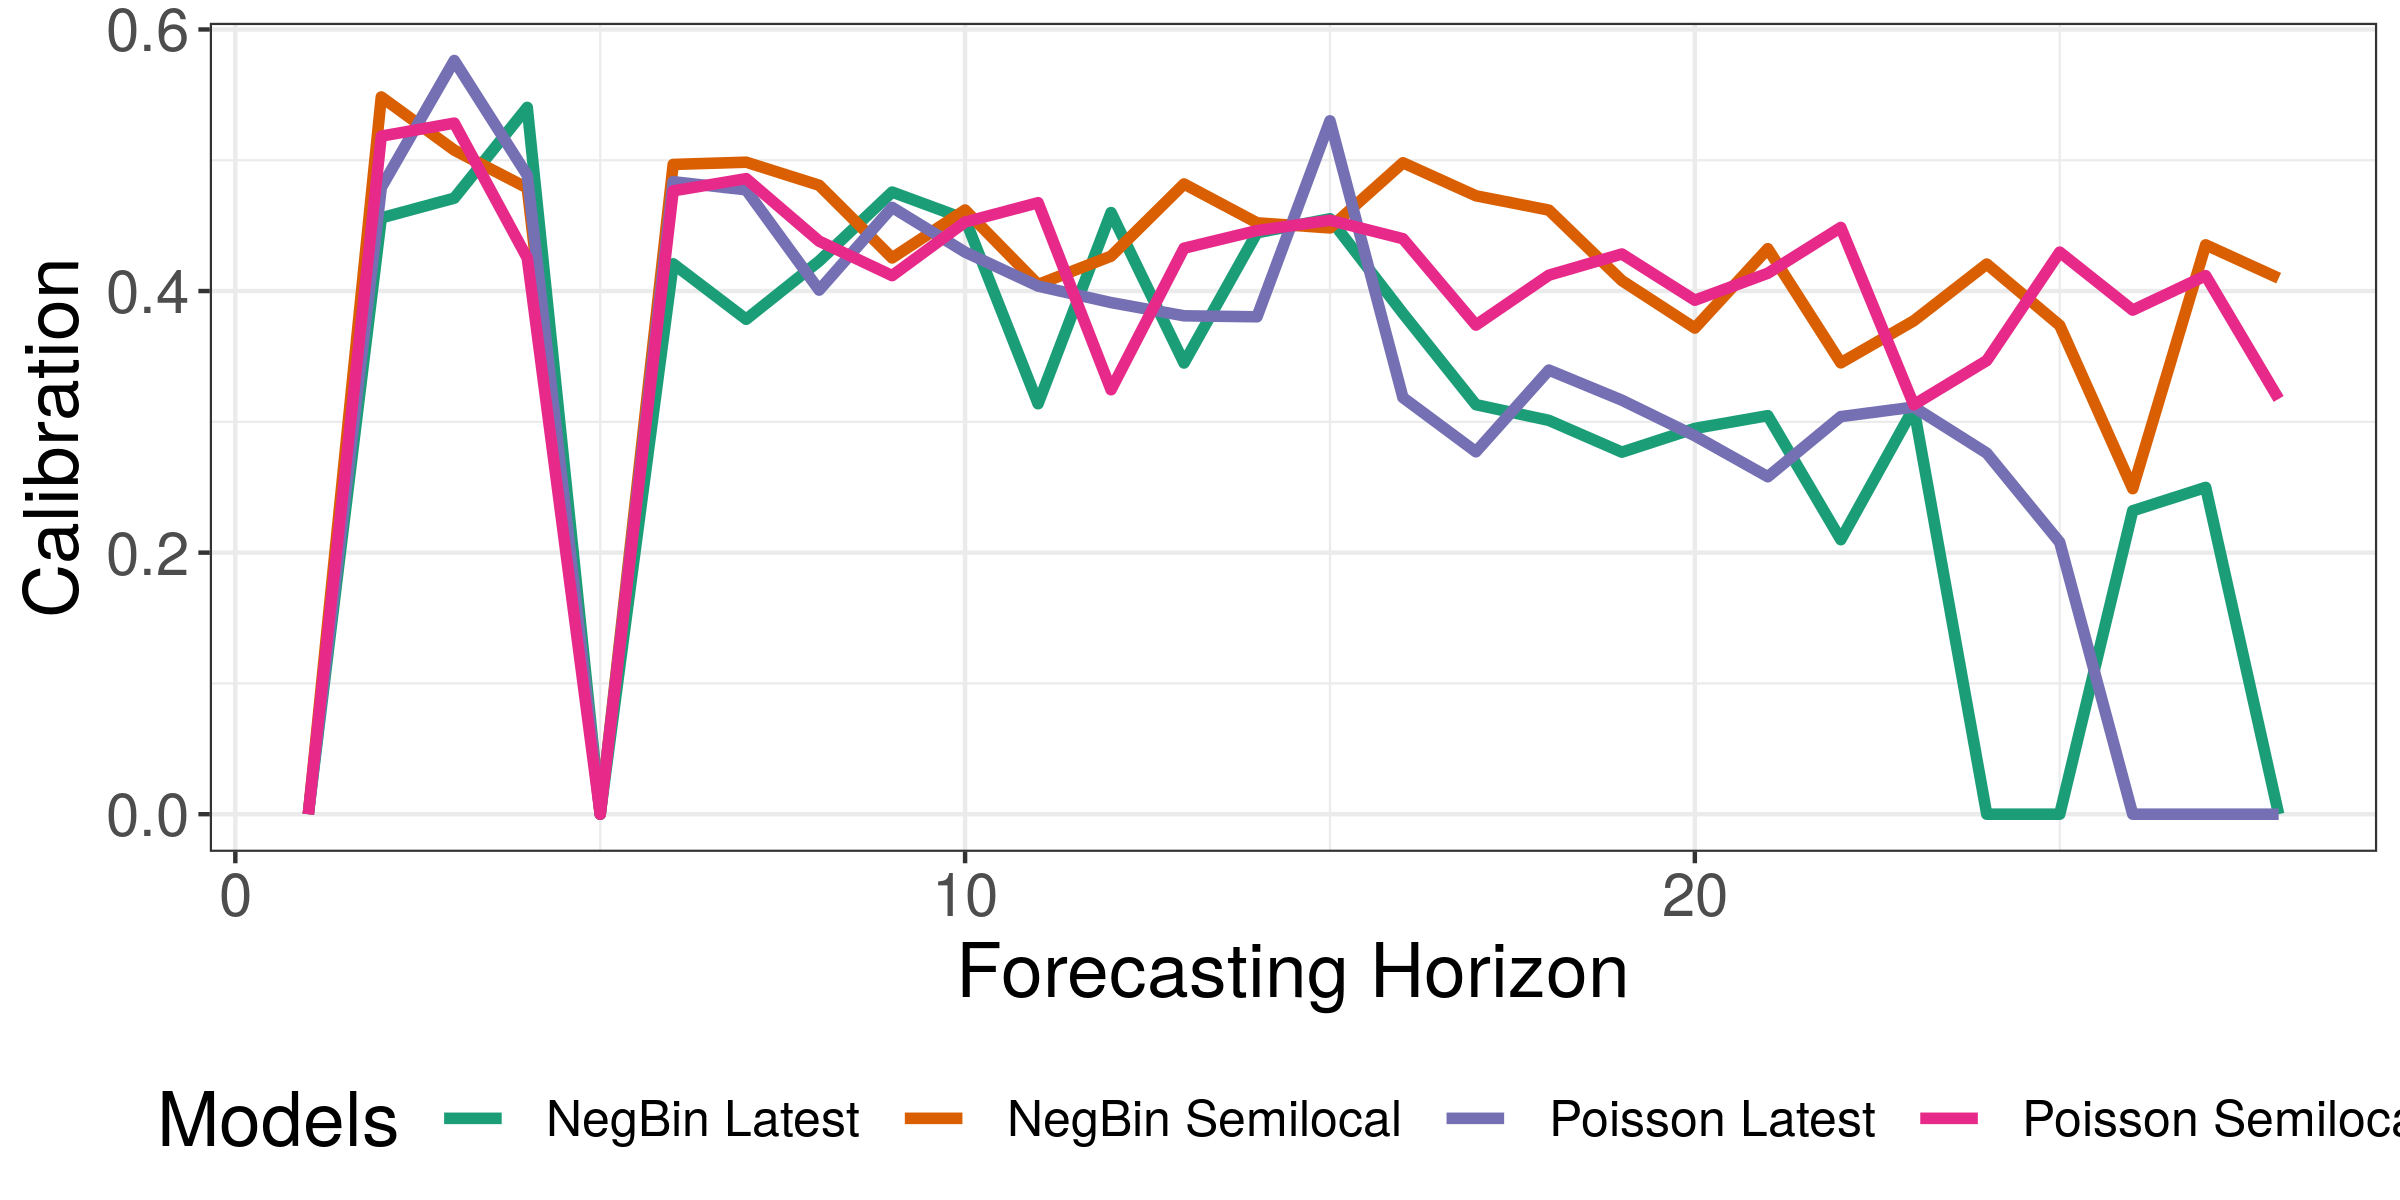
\includegraphics[width=\linewidth]{../output/Tchomia_calibration.png}  
  \caption{Calibration p-value}
  \label{Tchomia_scores_2}
\end{subfigure}

\begin{subfigure}{0.5\textwidth}
  \centering
  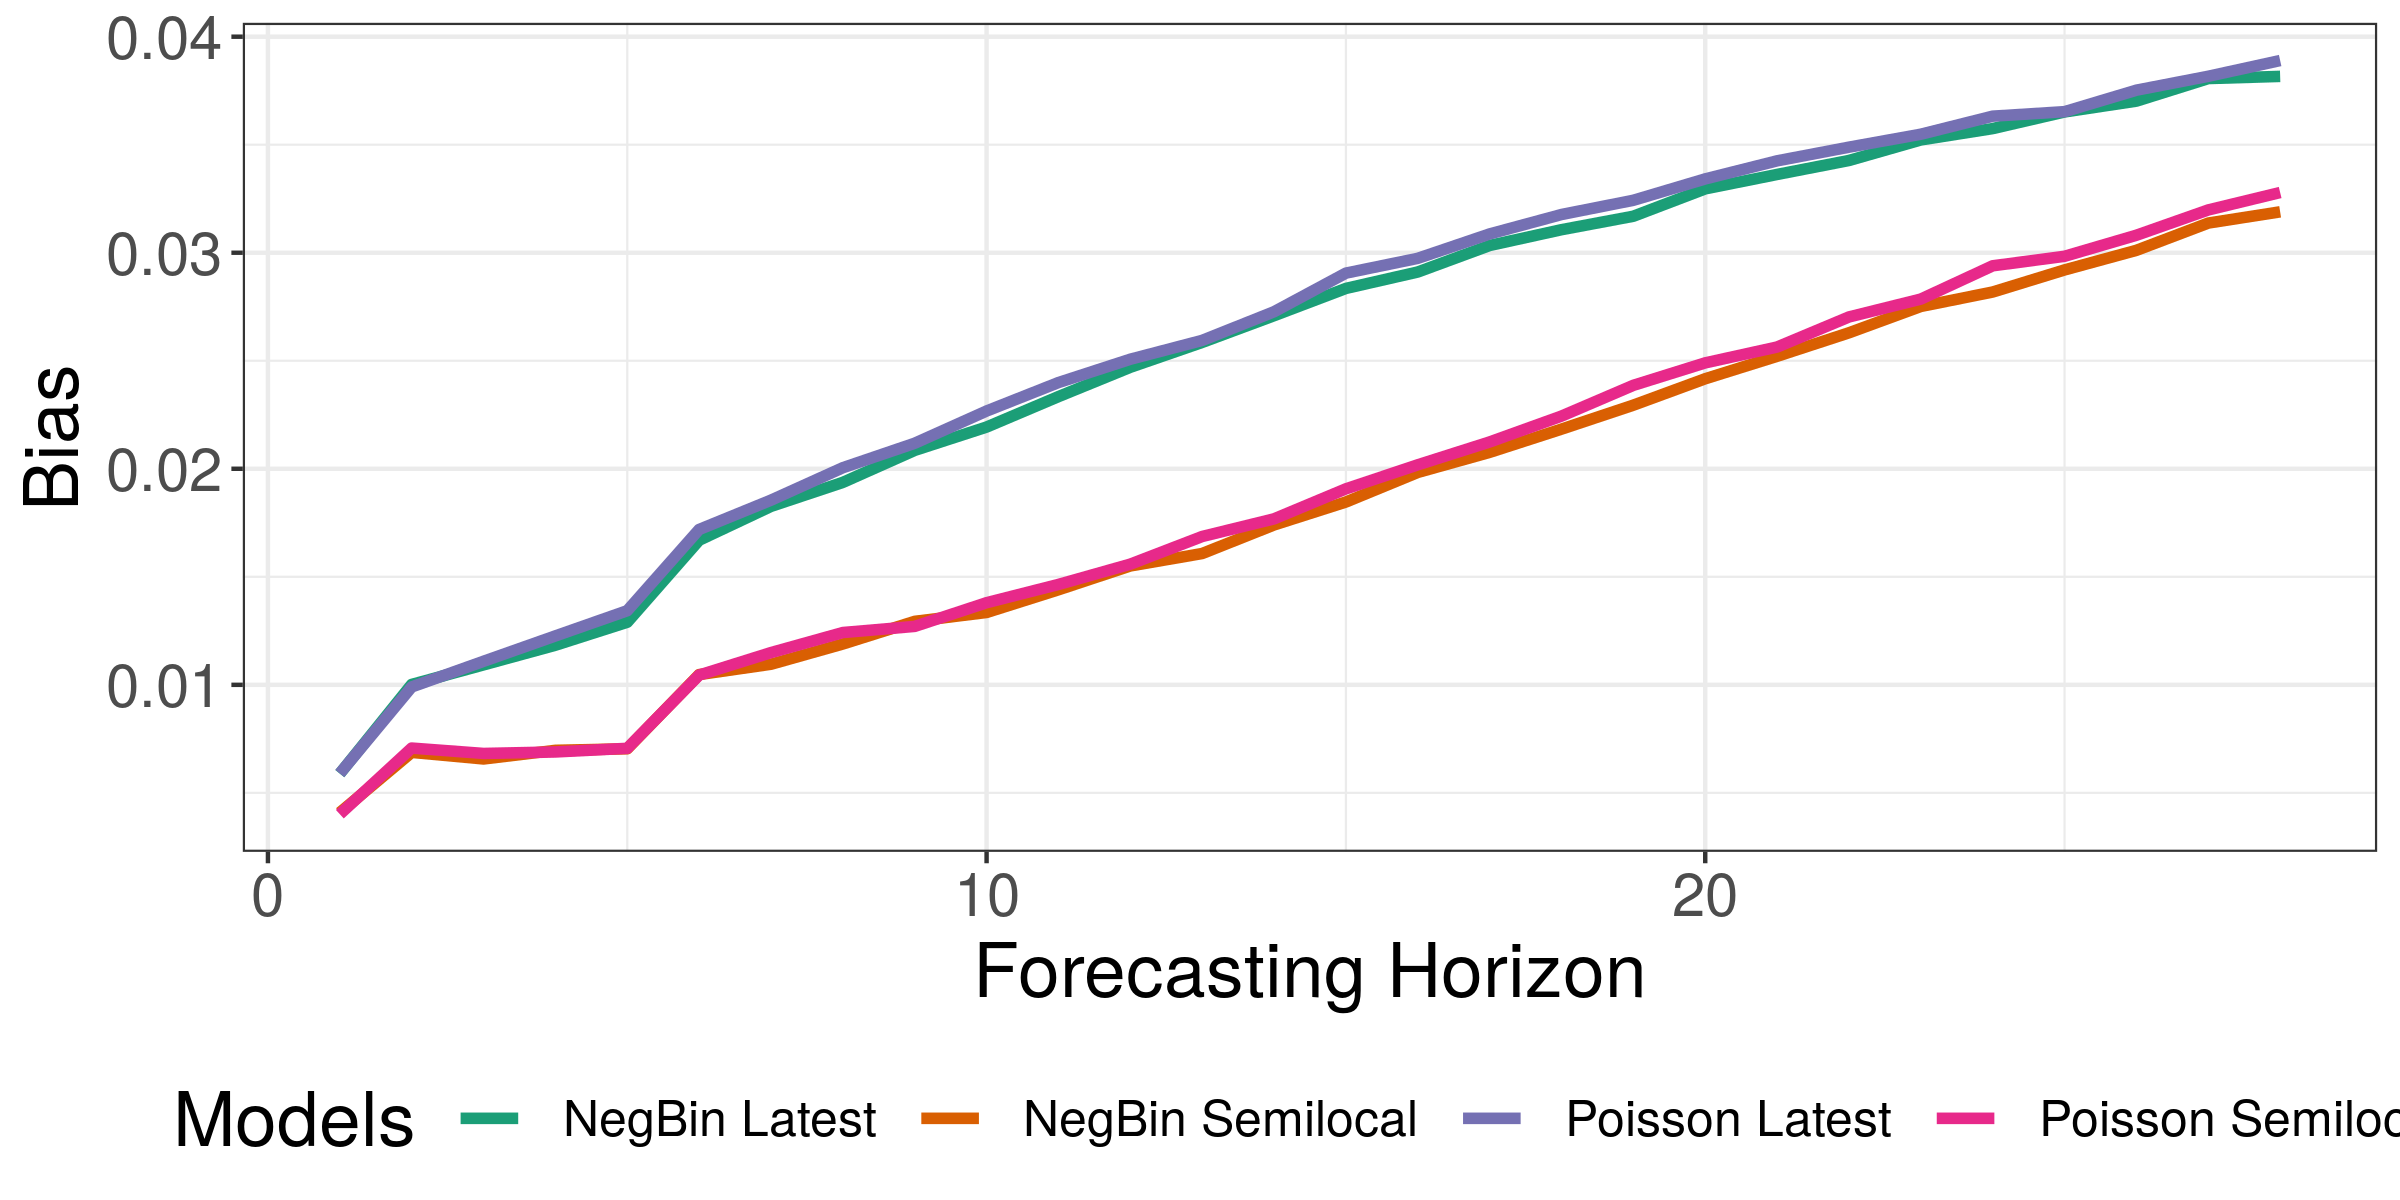
\includegraphics[width=\linewidth]{../output/Tchomia_bias.png}  
  \caption{Bias}
  \label{fig:Tchomia_scores_3}
\end{subfigure}
\begin{subfigure}{0.5\textwidth}
  \centering
  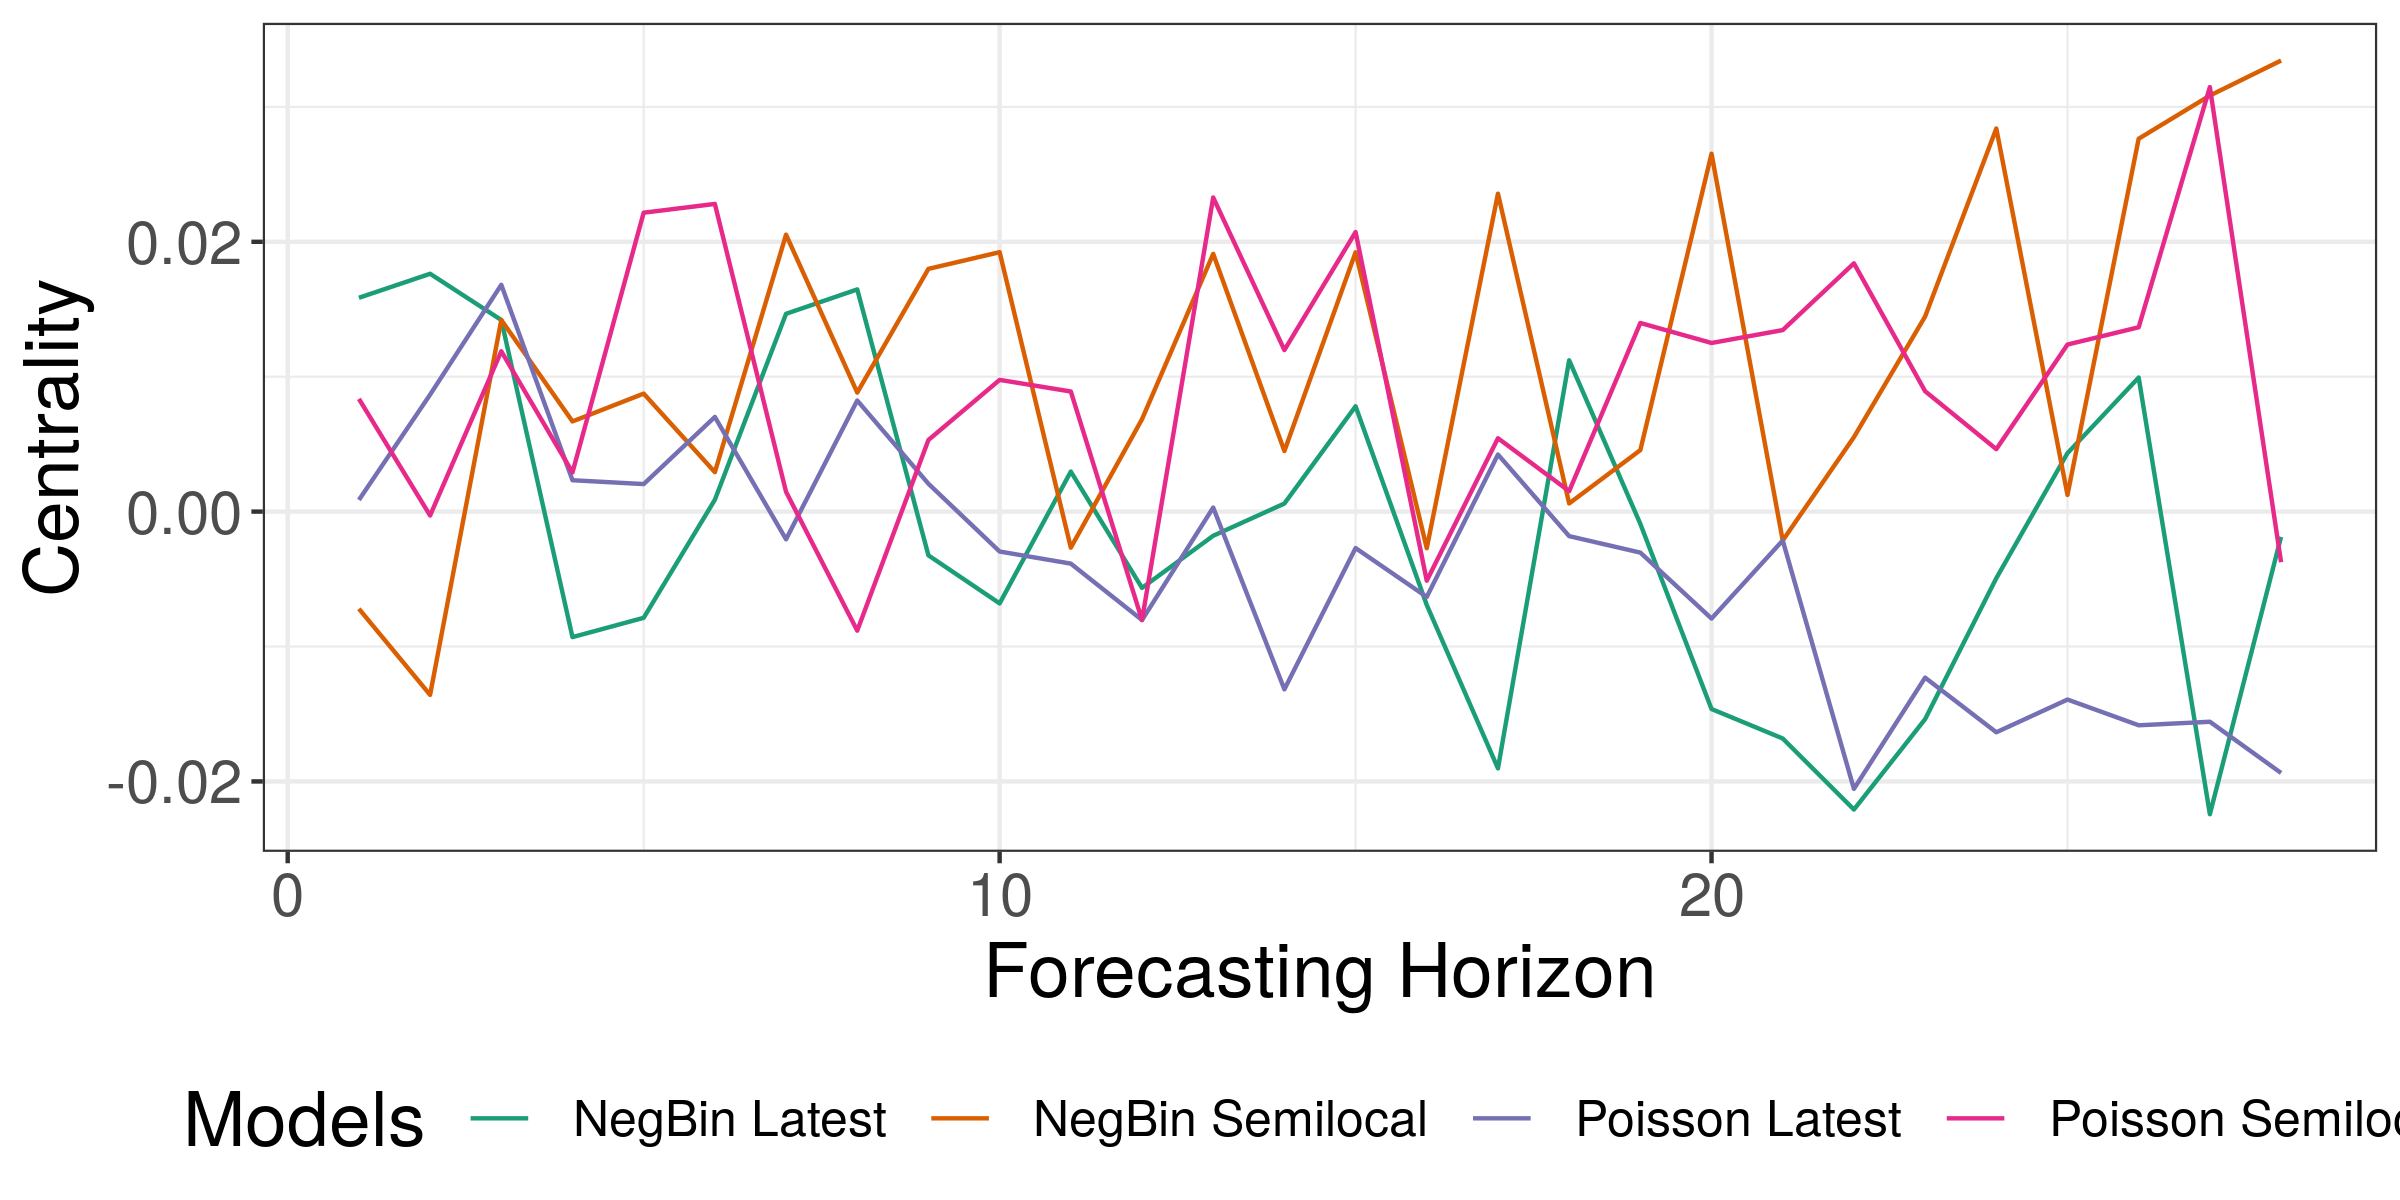
\includegraphics[width=\linewidth]{../output/Tchomia_centrality.png}  
  \caption{Centrality of PIT values}
  \label{fig:Tchomia_scores_4}
\end{subfigure}
  \caption{Scores for Tchomia as a function of the forecasting horizon.}

  \label{fig:nat_scores}
\end{figure}
